\section[Unbalance compensation with asym. inverter]{Voltage unbalance compensation with optimization based control algorithm and asymmetrical inverter structure}\label{VUB:sec:Compensation}

\hlc[PT]{This chapter describes the compensation of voltage unbalance (VU) of an unknown low voltage domestic network, with a current source power electric device, utilizing a PV power source and a lithium battery. The goal is, to reduce the VU on the network utilizing the limited resources, what the PV unit and the stored energy has to offer. With this in mind, the device is connected to any three phase four wire 400V connection point, and based on only on the measured network voltage, shall formulate such constrained harmonic current waveforms, that results in unbalance reduction based on the prescribed const function ($VUF$, or $G$, described in} \oldref{VUB:sec:Geom})\hlc[PT]{. Keep in mind, that the network transformer station's current and other properties, as well as the number and nature of the connected household size loads, and the network topology is unknown for the device. Furthermore, the loads connection and disconnection patterns (as such the network impedance) are time variant, with unknown stochastic distribution function.}\\
\hlc[PT]{Throughout the chapter, first the control problem shall be analyzed in detail, and the constraints and scope the formulation is operated with. Next the power electronic device's topology, and capabilities shall described, with a possible use case measured on a real connection point at the campus laboratory. Next in section} \oldref{VUB:sec:Optimization} \hlc[PT]{is the description of the optimization based algorithm's is written, and the argumentation why the particular method was used, and why is it suitable for the control problem previously outlined. The chapter closes with the simulation results performed in Matlab/Simulink and the discussion on the performance results, and the comparison of the device's operation modes.}
    %%
 %First the networks structure shall be described, the power electrical device is connected to, as a household supplying, renewable utilizing device, followed by the aforementioned device's topology and control shall be presented based on the geometrical voltage unbalance norm (described in section \ref{VUB:sec:Geom}), with the performance results on an unbalanced network. It shall be shown, that it is possible to formulate some power quality related aims, or demands for the domestic size generator units implemented in a complex power electrical system, capable of supplying a household, with both renewable and network supplied energy, and lowering voltage unbalance as well, considering a network with unpredictable impedance.

\subsection{Problem statement}\label{VUB:sec:Statement}

    The network, the proposed VU compensator supposed to be connect, is a three phase four wire low voltage domestic transformer area. depicted in Figure \ref{fig:network}. As such, the overwhelming loads, are assumed as single phase, with resistive (e.g.: heaters) inductive (e.g.: motors) and capacitive (e.g.: chargers) properties as well, while some of them are symmetric three phase ones (e.g.: induction ovens, compressors, inverter fed motors).

    \begin{figure}[!ht]
    \centering
    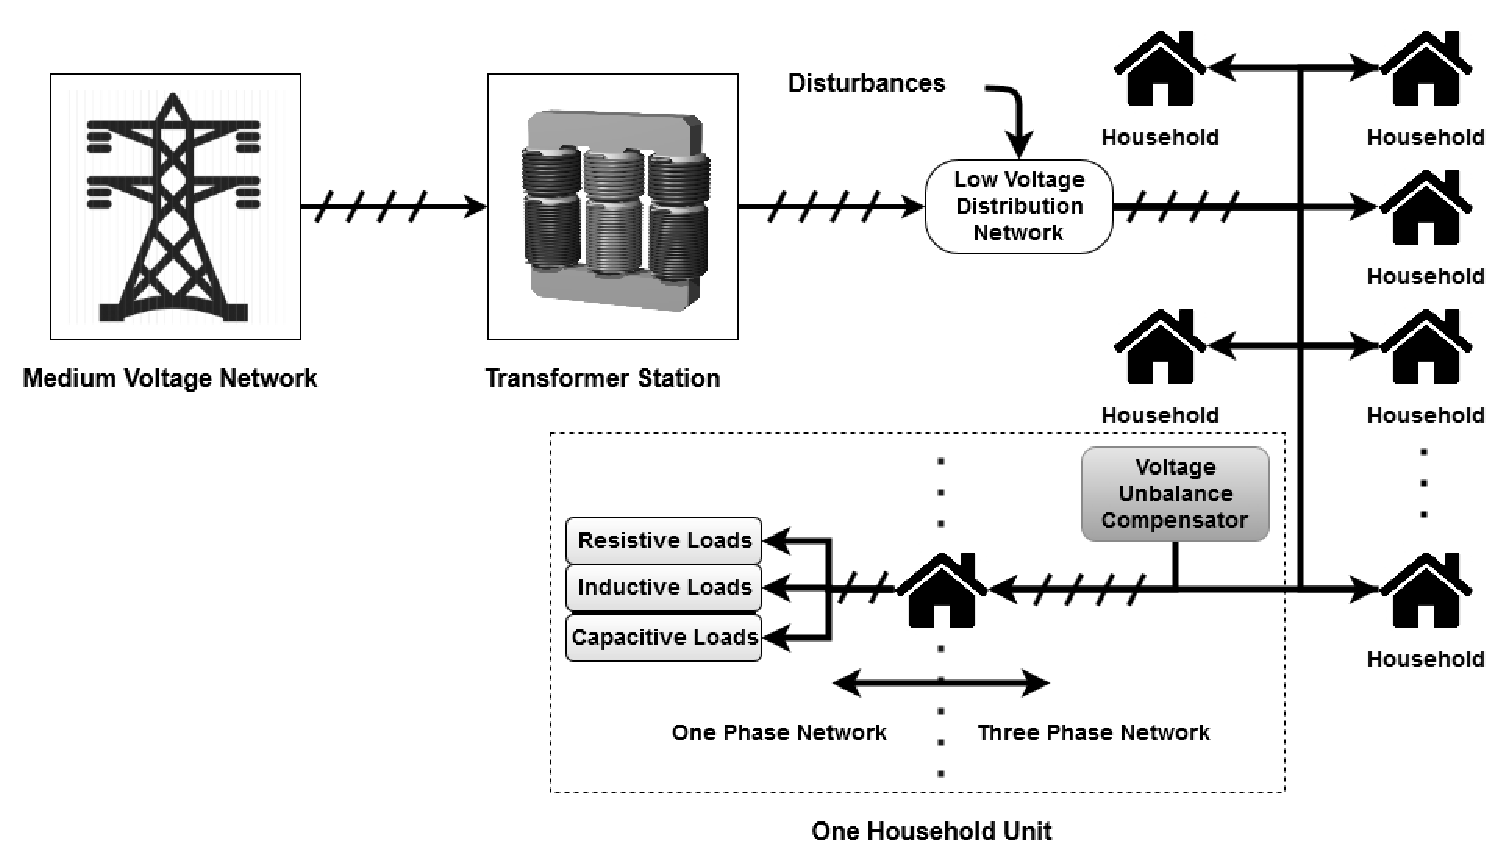
\includegraphics[width=\textwidth]{Unblance_EPS_Pics/network_gray.eps}
    \caption{The simplified structure of a three phase four wire low voltage network. Several regular households are representing the main loads, and connected with power line sections, subject to inductive and resistive disturbances and capacitive couplings. Domestic powerplants may connect to any connection point within the low voltage section, via an appropriate inverter - either to the three phase sections using a three phase inverter or to a single phase using a single phase inverter.}
    \label{fig:network}
    \end{figure}

    Due to the unregulated, and uneven load, or (with the emergence of affordable PV stations) possible domestic powerplant distribution, the voltage and current unbalance present in the network causes additional power loss inside the medium voltage/low voltage transformer and in the transportation line wires too. It also has undesired effects in certain three phase loads, mainly rotating machines where it causes torque reduction and pulsating torque effect. Large scale unbalance can also activate automatic protection functions of electricity dispatch system causes power outage. These negative effects lower the electric power quality and rises the cost of electrical energy and rises the carbon footprint of our everyday life, and also undesirable for the customers and adds maintenance cost to the service provider.\\
    \hlc[PT]{This chapter's aim to propose a model and control scheme for a three phase instrumentation, which can compensate voltage based unbalance, and as such lower the power losses and increase power quality, not only at the domestic connection point but in the whole low voltage transformer area without prior knowledge of the network's topology, it's connected load's, or the transformer characteristics. Also doing so with the energy provided by a PV source and stored energy in a battery bank, or in some cases, via 'zero balance operation' where the power reserves are empty.}\\
    \hlc[MA]{The voltage network, as the indicator of unbalance is assumed to react to the controlled current injection} \ref{eqn:VU_netwfcn}:

    \begin{equation}
    \label{eqn:VU_netwfcn}
    \begin{array}{rcl}
    V_{abc}=f_{grid}(i_{abc})\\
    \end{array}
    \end{equation}

    \hlc[MA]{where $f_{grid}$ represents the unknown function of the network at the device's connection point, $V_{abc}$ is the measured network , and $i_{abc}$ is the current injected or consumed by the device.} \hlc[MA]{As} \ref{eqn:VU_netwfcn} \hlc[MA]{suggests, the injected current waveform's effect is assumed to be immediately observable as the change of the network's voltage, however, the uncertainty of $f_{grid}$ does not make the approach so straightforward as with exact, or semi-exact model based controllers. Finally, the cost function is naturally comes form the formulation of the VU norm of choosing:}

    \begin{equation}
    \label{eqn:VU_costfcn}
    \begin{array}{rcl}
    VUF=f_{VUF}(V_{abc})\,or\,G=f_{G}(V_{abc})\\
    \end{array}
    \end{equation}

    \hlc[MA]{where $VUF$ is the state of the art, and $G$ is the proposed geometrical indicator of VU. $f_{VUF}$ is described by} \ref{BASICUNB:equ:VUF}, and $f_{G}$ is described by \ref{equ:geom}. \hlc[MA]{The scope of analysis is limited to only these two norms, but the principle works with any valid VU indicators of choice.}\\
    The above problem statement specifies the scope solution space together with the solution method. \hlc[PT]{It can be observed in Fig. }\ref{fig:mininetwork}\hlc[PT]{, that the system of interest is the power grid with all the unknown stochastic and nonlinear phenomena, represented as a black box model, with limited observability through the measured voltage ($V_{abc}$). It is worth mentioning, that current measurement is only available at the poles and inside the device, since after the household meter or at the transformer poles, current measurement would be expensive, although the global network VU is observable at this connection point also. The input to the system are current signals (one current in the single phase case and three in the three phase setup), which are naturally constrained by the available energy of the household, stored in a battery pack or momentarily generated by the wind or solar generator unit. The response of the system can be either the current or the voltage measured at the connection point of the inverter unit, however, the general legal regulations only allow voltage measurement for consumers.}\\

     \begin{figure}[!ht]
    \centering
    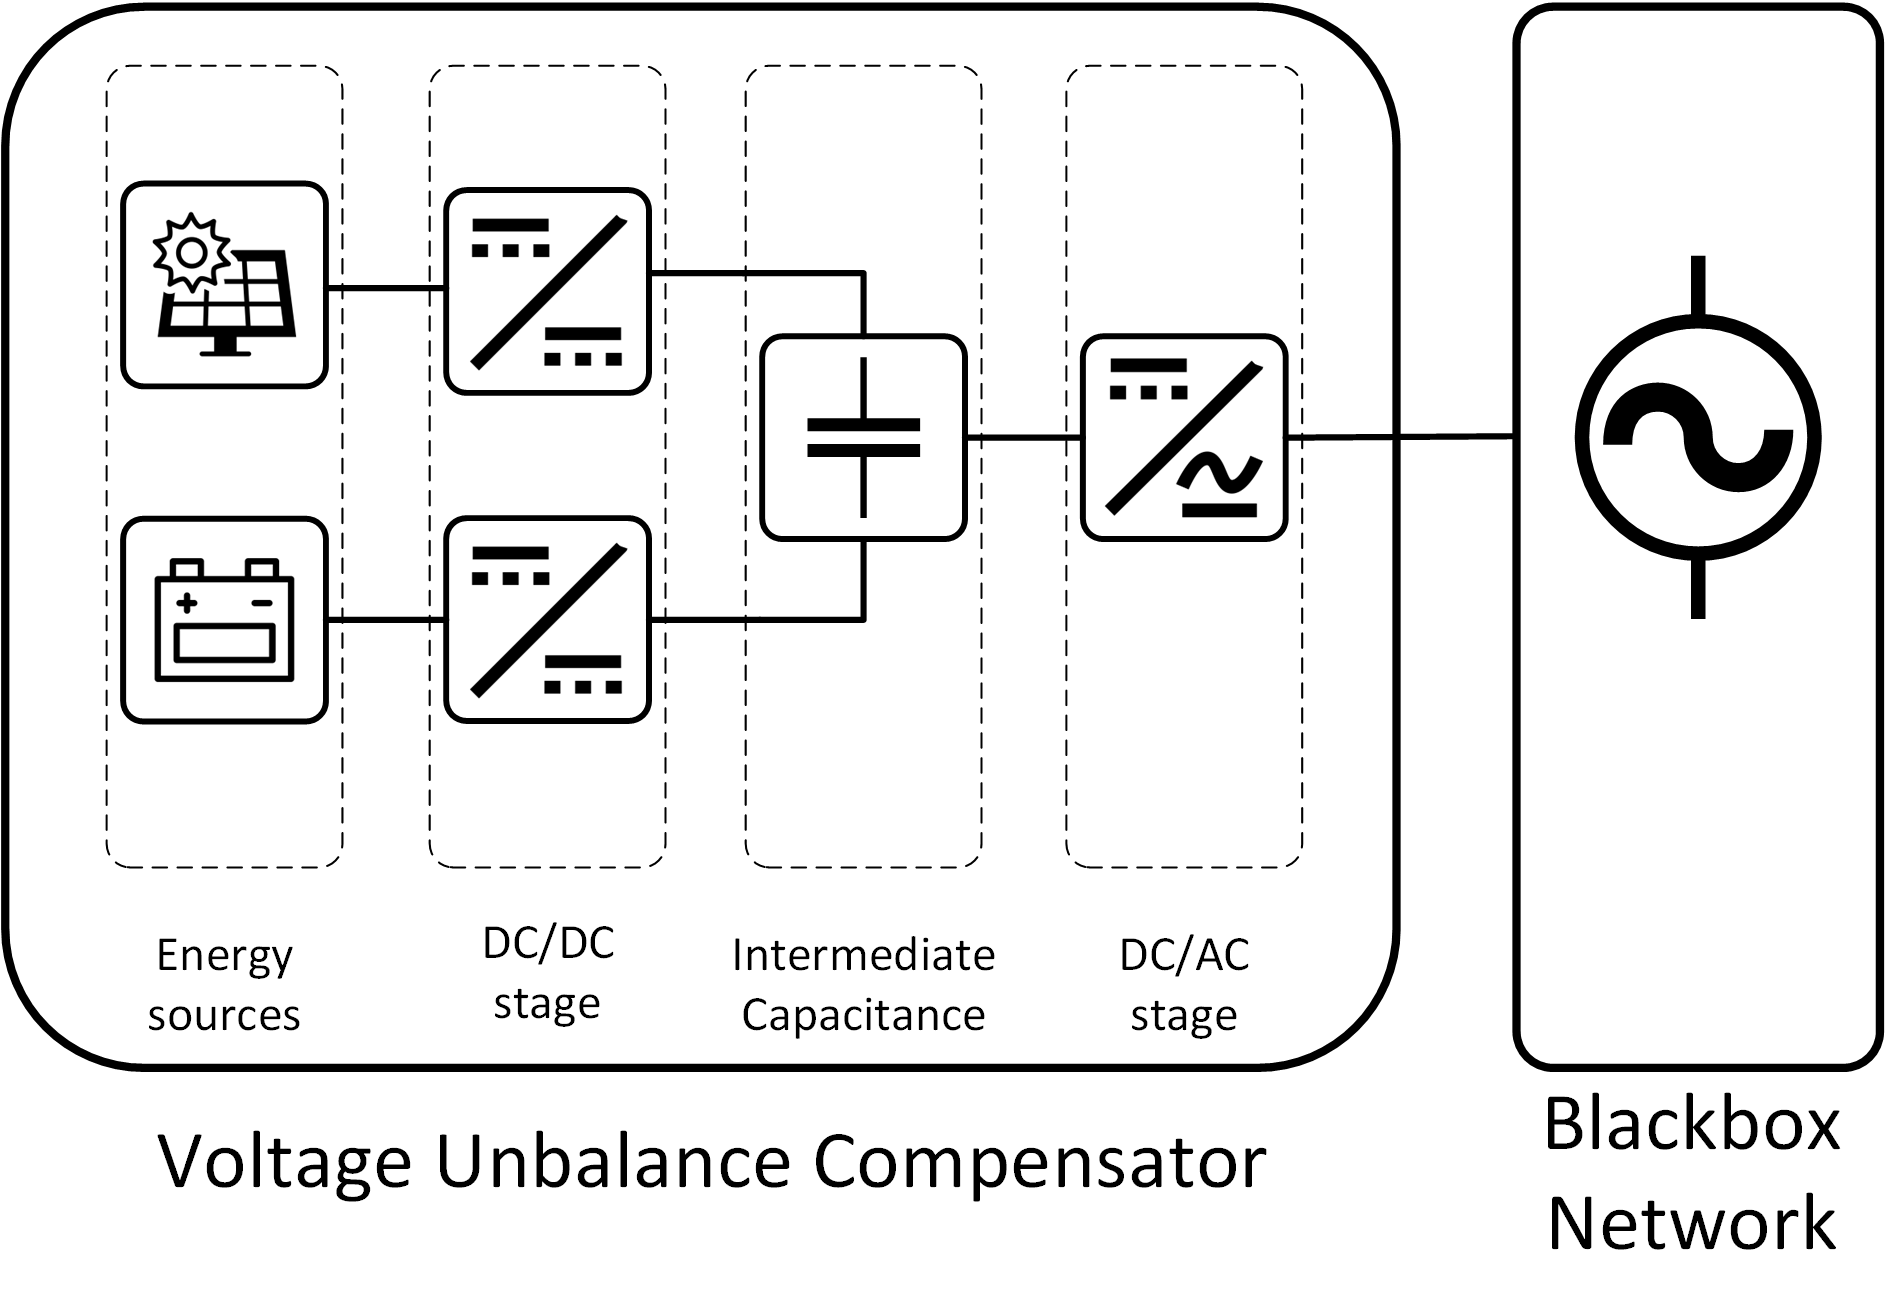
\includegraphics[width=.6\textwidth]{Unblance_EPS_Pics/VUCompensator_minichart.png}
    \caption{Simplified compensator perspective and overview.}
    \label{fig:mininetwork}
    \end{figure}


    The difficulty of the control problem comes from the fact, that there are no mathematically tractable models of the network can be generated because of its unpredictable and nonlinear features. This means, that in these conditions only black-box methods can be applied for this system.
    For the control aim it is a natural choice to minimize the actual voltage unbalance of the low voltage local transformer area measured (or calculated) at the connection point of the inverter. Several optimization based methods are available for such kind of optimal control problems, e.g. \cite{gorbe2012reduction} where the only bottleneck is the computational efficiency since the implemented controller has to run on the commercial inverter's hardware (digital signal processor unit).

    \subsection{Optimization based control algorithm}\label{VUB:sec:Optimization}

        Ideally, the point $\textbf{x}^q$ corresponding to the local minimum, which can be calculated from the negative gradient $\nabla f(\textbf{x})$, that gives the value and direction of the corresponding step in the parameter space, as such making the optimization straightforward. The next step is made in the direction of gradient with the proper sign. Most of the time, this sequence of steps, converges to local multivariate extreme value $\textbf{x}^q$ of the function \ref{eqn:contstruct1}.

        \begin{equation}
        \begin{array}{rcl}
        \label{eqn:contstruct1}
         \textbf{x}^{(q)}&=&\textbf{x}^{(q-1)}-t_q\nabla f(\textbf{x}^{(q-1)}),\\
         %q&\in&\mathbb{N},\\
         \end{array}
        \end{equation}

        where $q\in\mathbb{N}$, and $t_q$ resembles the step time of the algorithm.%
        Unfortunately, the controlled electrical system is described by multivariate non-linear differential equations, the optimization of which is infeasible to derive using the differentiation of an error function. Therefore, the optimization methods based on direct differentiation are not applicable. In such cases, when high computational power is needed for performing long time-consuming simulations, the so called asynchronous paralell pattern search or APPS method can utilized.\\
        \hlc[PT]{There is a long history for identifying VU on the network as presented in section}\oldref{BASICUNB:sec:DefinitionsofUNB}\hlc[PT]{ As such the basis of the }\hlc[MA]{cost} \hlc[MA]{function is well defined in} \ref{eqn:VU_netwfcn}. \hlc[PT]{Since the network is assumed not only non linear and  time variant, with unknown stochastic distribution function, the mathematical representation of the network from the device's perspective would be a difficult task. As such the network's voltage response to a certain current injection is hard to predict, and could make the situation even worse, distorting the voltage phasor even further. Wit this in mind regular PID controllers are not sufficient, although there were attempts to solve similar control problems with artificial intelligence} \cite{el2011active}.\\
        For this purpose I choose an asynchronous parallel pattern search method (APPS) to control our scenario \cite{hough2001asynchronous}, \cite{kolda2003understanding}. The methodology and formulation of the APPS method is described in more detail in section \oldref{BASICUNB:sec:APPS}.

        It can be assumed, that the network function $f_{grid}$ from \ref{eqn:VU_netwfcn} is hard to estimate, as such, the best approach is to use parallel computing environment to solve the problem, instead of function evaluation. Since $f_{grid}$ is continuously differentiable, it can be further assumed, that it's gradient $\nabla f_{grid}$ unavailable and also unreliable to approximate to the non linear time variant network operation. For this type of problems, so called pattern search methods are one possible solution, since they neither require nor explicitly estimate derivatives.  Pattern search methods also have a long history of success when applied to non linear problems \cite{hough2001asynchronous}.\\
        With this in mind the list of processes which could be parallelized, comes from shape of the voltage phasor itself (observed in Fig. \ref{fig:threephase}). The ideal phasor is deviating in terms of voltage amplitudes and angles. As such, if the first phase $V_a$ is is locked by angle, it can be assumed, that the ideal phasor can deviate by two phases and three amplitudes. As such the search algorythm has five processes (or axes) to optimize along. Basically the general strategy for the APPS method, from a single process perspective follows: %\textcolor{red}{Attila, az algoritmust nézd át kérlek hogy konzisztens-e!}
        %
        \begin{algorithm}[H]
        \SetAlgoLined
        %\KwResult{Write here the result }
         $\textbf{x}_i^0=0$, $\Delta_i^0=0, d_i^{(q)}=1$\;
         \While{$f_{grid}(\textbf{x}_i^{q}+\Delta_i^{(q)}d_i^{(q)})\neq0$}{
          $N^{(q)}=f_{grid}(\textbf{x}_i^{(q)}+\Delta_i^{(q)}d_i^{(q)})$\;
          $d_i^{(q)}=0.5(sign(N^{(q-3)}-N^{(q-2)}+sign(N^{(q-4)}-N^{(q-3)})))$\;
          $\Delta_i^{(q)}=n_{i}N^{(q-1)}\Delta_i^{(q-1)}+\Delta_i^{(q-2)}+m_{i}N^{(q-1)}$\;
          \eIf{$f_{grid}(\textbf{x}_i^{(q)}+\Delta_i^{(q)}d_i^{(q)})<f_{grid}(\textbf{x}_i^{(q)})$}{
          $\textbf{x}_i^{(q+1)}=\textbf{x}_i^{(q)}+\Delta_i^{(q)}d_i^{(q)}$\;
          $I_{APPS}=f_{current}(\textbf{x})$\;
          $I_{abc}=\frac{V_{abc}}{R_{virt}}f_{inter}(V_{inter})+I_{APPS}$\;
           %<bradcast new result of $f_{grid}$ to other processes>\;
           }{
          }
          }
         \caption{Asynchronous Parallel Pattern Search}
         \label{algo:APPS}
        \end{algorithm}

        where $f_{grid}$ representing the multi variate voltage response function of the grid of which cost ($VUF$ or $G$)
        function could be calculated, based on current injection, $f_{current}$ updates and formulated the three phase current waveform based on the amplitude and voltage values $\textbf{x}$ vector represents, and $f_{inter}$ represents the intermediate buffer capacitance's PID voltage controller. The function arguments are $\textbf{x}_i$, the actuator for the $i^{th}$ process aka. the amplitude or phase of the three phase current phasor, needs to be applied on the system, for VU reduction. This value is later offsetted by the normalised value of internal capacitance, $V_{inter}$, and the scaled value of the network voltage $V_{abc}$ by a virtual resistance $R_{virt}$. Since the injected currents are synchronised via initial Fast Fourier Transformation (FFT), this operation could be performed. Furthermore, $\Delta_i$ the process step length aka. the value of the current vector's amplitude or angle needs to be changed for a successful step, and $d_i$ is the corresponding step's signed direction vector, which specifies the applied changes direction. Furthermore $N$ represents the chosen nor's value as the network's response to the current injection, and $n_i$, and $m_i$ are scaler gains for the corresponding process. The algorithm is initialised with $\textbf{x}_i^0=0$, $\Delta_i^0=0$ for a smooth start, due to lack of prior network knowledge.

        where $f_{grid}$ representing the multi variate voltage response function of the grid of which cost ($VUF$ or $G$)
        function could be calculated, based on current injection. The function arguments are $\textbf{x}_i$, the actuator for the $i^{th}$ process aka. the amplitude or phase of the three phase current phasor, needs to be applied on the system, for VU reduction, $\Delta_i$ the process step lenght aka. the value of the current vector's amplitude or angle needs to be changed for a successful step, and $d_i$ is the corresponding step's signed direction vector, which specifies the applied changes direction. Furthermore $N$ represents the chosen nor's value as the network's response to the current injection, and $n_i$, and $m_i$ are scaler gains for the corresponding process. The algorithm is initialised with $\textbf{x}_i^0=0$, $\Delta_i^0=0$ for a smooth start, due to lack of prior network knowledge.

        \begin{figure}[h]
        \centering
        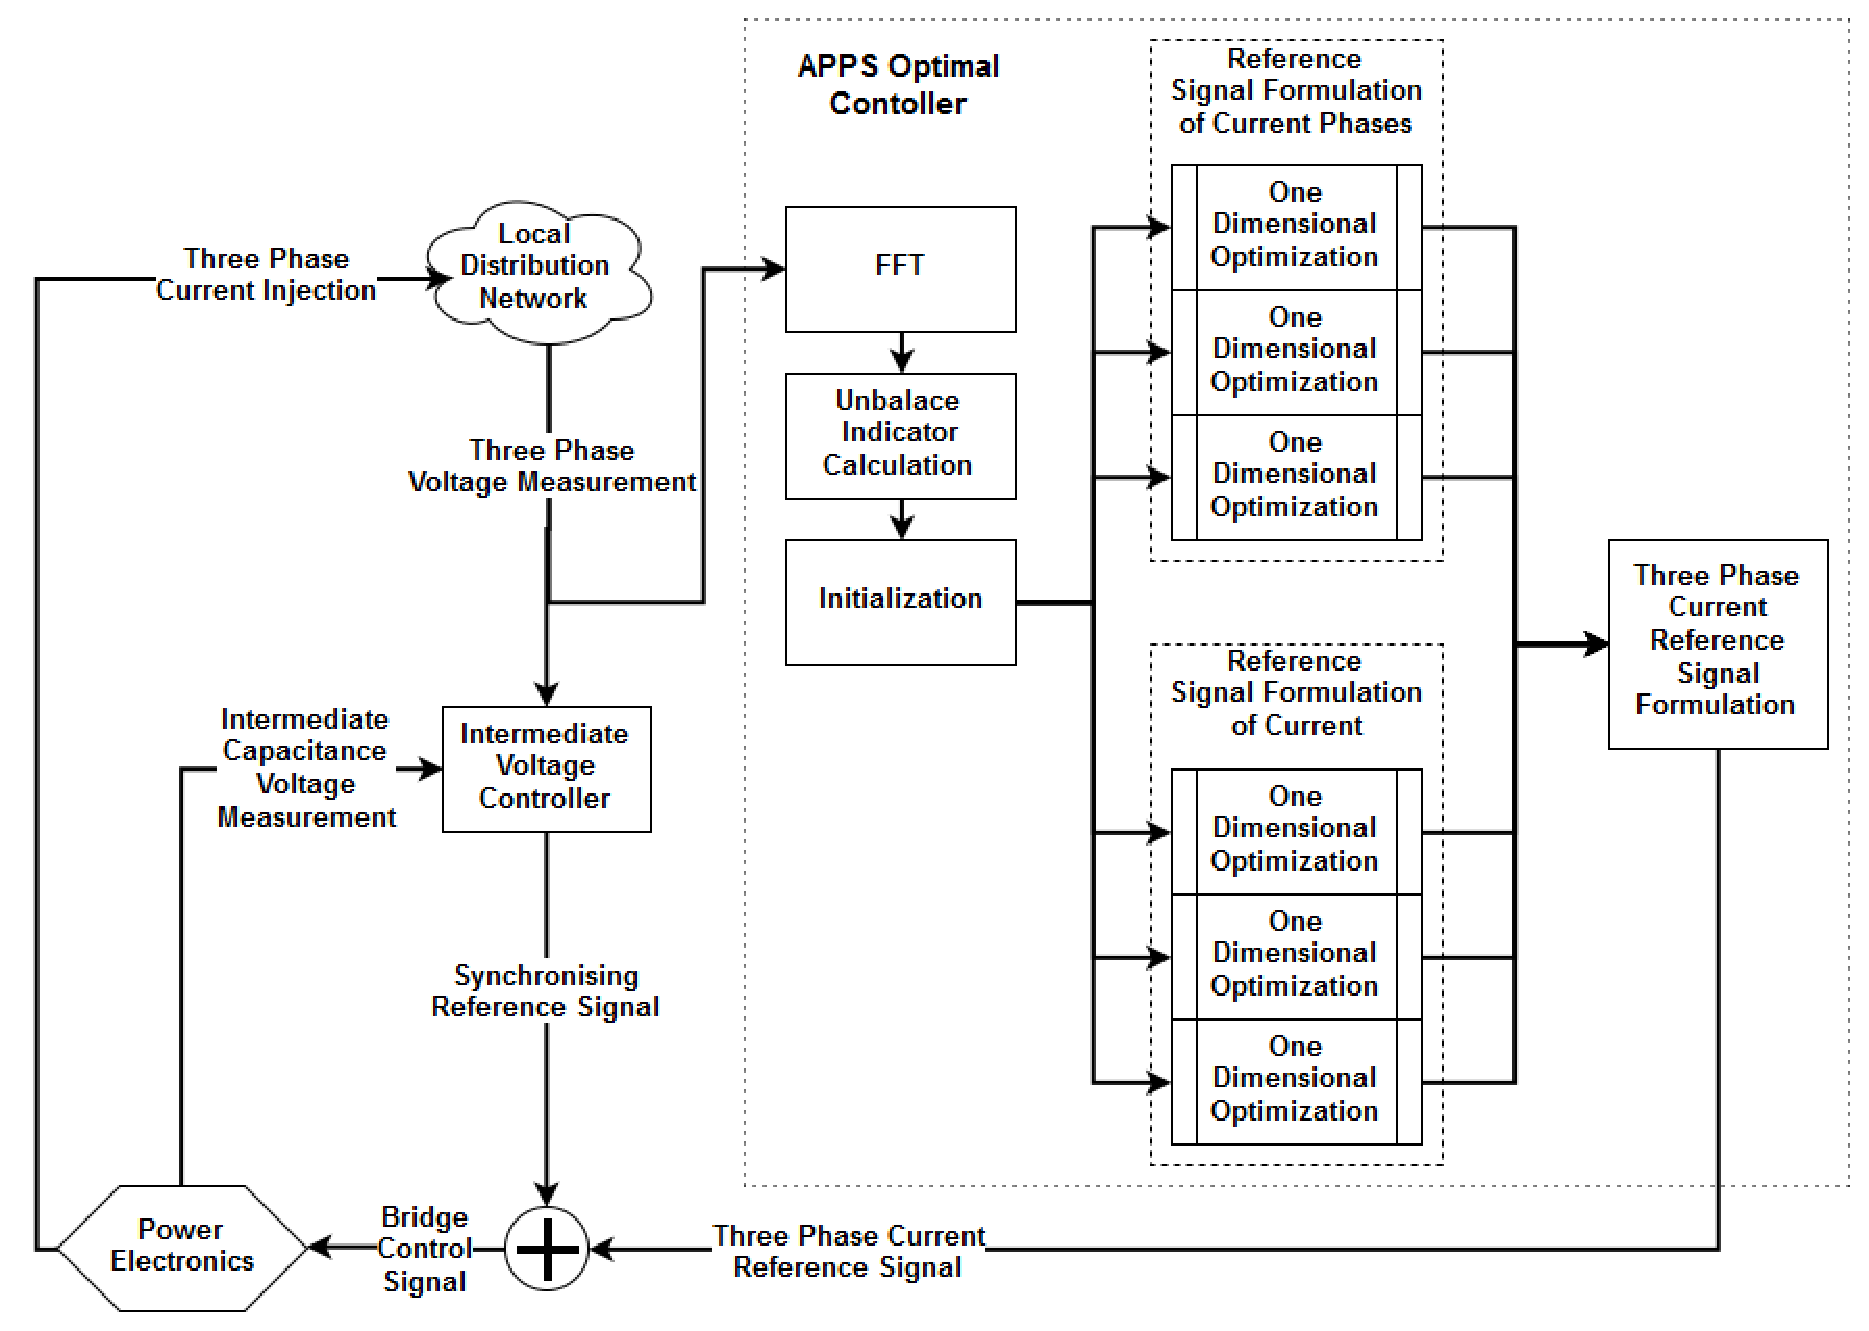
\includegraphics[width=0.95\textwidth]{Unblance_EPS_Pics/APPS_1_2_.eps}
        \caption{The optimization algorithm implemented for current control. A one dimensional linear optimization step is being solved in each dimension of the six dimensional parameter space, iteratively.}
        \label{fig:APPS}
        \end{figure}

        %\textbf{red}{régi részek:}\\
         The search pattern $p$ is based on the sampling of the error function (selected norm) on $f_{grid}$, and it corresponds to variables or subsets of variables in each point in the independent variable or parameter space. At the same time, the norm values at these points can be calculated independently if $\Delta_q>0$, using algorithm \ref{algo:APPS}.
				
        %\begin{equation}
%        \label{eqn:contstruct2}
%        \begin{array}{rcl}
%         \textbf{x}^{(q+1)}&=&\textbf{x}^{(q)}+\Delta_qd_i \\
%         \mathrm{if}&&f(\textbf{x}^{(k)}+\Delta_qd_i) \leq f(\textbf{x}^{(q)}),\\
%         %q&\in&\mathbb{N}\\
%         \end{array}
%        \end{equation}

        The parameter is $\textbf{x}^q\in\mathbb{R}^n$, and the \hlc[PT]{initial} search pattern $\textbf{p}\in\mathcal{D}={d_1,...d_n}$ is taken from a predefined finite set\hlc[PT]{, and updated every iteration}. In this case, the error function values of $N$ should be calculated for each pattern $\textbf{p}$ in the set $\mathcal{D}$. As the competing directions are different, if there is not enough computing power available for direction vector $\textbf{p}$, synchronization should not be maintained. In this case we are talking about the asynchronous case. In the case of our controller, an individual $\textbf{p}$ vector is defined for each output variable, and the optimization was performed in each direction asynchronously and shifted in time. Most likely, the error function has a single local minimum as a symmetric amplitude and phase values. Approaching the minimal value of norm, the controller uses adaptive increments that are proportional to the norm itself. Because of the complex interactions between the components of the controller, only one parameter is changed at a time, even if the values of the amplitude and phase components in specific time slot changes. The algorithm moves along the six axes of six separate time slots close to the local minimum of the error function.\\
        Unlike other similar approaches, e.g. \cite{segui2007approach}, the explained optimal controller does not rely on a measured current signal (which varies according where the measurement took place on the grid and renders the global optimization unreliable) but rather measuring and analyzing the voltage unbalance via the proposed indicator and optimizes the voltage shape, the latter of which depends on the nonlinear distortion of the whole low-voltage transformer area and determines additional power losses. The controller's performance was compared to a non compensated network, and a network consisting synchronized symmetric power intake from a regular inverter.\\
        In each iteration only one physical value is changing on the six dimensional parameter field, which consists of the three amplitude and three phase values. If the change effects with cost function reduction (the reference norm's normalized value), the controller holds the new value of amplitude or phase for the controlled current sources (Figure \ref{fig:APPS}). The advantage of this controller structure that is not necessary to know the controlled value's behavior well, like we could not determine the number and type of the other loads on the network \cite{Neukirchner2015}. There are however two disadvantages. First is the low speed of control, due to the several necessary iterations (depending on the circumstances) to find the optimal directions in the parameter space, and the serial nature of interventions and norm calculations. The second comes from the method itself since the controller may stuck in local minima.

    \subsection{Asymmetrical inverter topology}\label{VUB:sec:Inverter}

    The applied structure based on a full bridge IGBT structure used in single phase current injection. Three different IGBT full bridge were connected at the output point, thus our structure has three phase and neutral connection too, to carry out any current form. The disadvantage of this structure is that it needs 12 IGBTs in the output stage as opposed to the 6 IGBTs needed for a classical full bridge structure and needs three galvanically isolated direct current (DC) voltage source for feeding.\\
    For the sake of completeness an asymmetrical inverter was developed in simulation environment, which is capable of carrying out the specified control task. The renewable energy injection is realized increasingly, and applied directly to the three phase low voltage grid  with a domestic size photovoltaic power plant as source of power. This can reduce the voltage and current unbalance caused by the stochastic power production of wind and solar sources. More and more manufacturers produce three phase grid synchronized inverters from 5\,kW size. These equipments implement accurate symmetrical current feed with a standard three phase full bridge structure, consists of six Isolated Gate Bipolar Transistors (IGBT). The demand is to employ a current source single phase structure with aforementioned controllable switches in section \oldref{BASICCSR:sec:CSI}. This is a standard structure suitable for symmetric harmonic current injection. It has limited capacities to inject not totally symmetric 3 phase current time functions, but Kirchhoff's current law permits only constant zero-sum current time functions injected with this structure. There are examples with this type of asymmetric current injections in the literature \cite{lee2009new}.\\
    This type of current injection has limited compensation capacity and this is not enough in most asymmetric production and load cases. In our case we need more general, not specific asymmetric current waveforms, because the proposed control aim assumes the ability of injecting non zero-sum currents. This needs special inverter design structure. We need zero line connection for the differential current. One of the possible solution is to use 3 different full bridge single phase current inverters to supply each phase of low voltage transportation lines \cite{Patnaik2013topologies}. This way it is most sufficient to use bi-directional power flow, with galvanic decoupling, but with a current controlled fashion (shown in section \oldref{BASICCSR:sec:CSI}).\\
    This isolation can be reached  with using isolation transformers in the supply side. But we prefer to use it a complex energetic system with specific inside true DC bus system fed from Photovoltaic panel or batteries. We have to isolate at least 2 full bridges with two way DC-DC converters (described in section \oldref{BASICCSR:sec:DCDC}). This can complicate the physical realization but easy to simulate with two controlled power source. Other possible easy to realize solution to isolate the full bridge outputs  connected to three phase lines with isolating transformers. It is recommended due to electric shock protection reasons. Our distant aim to compensate other operational type line failures, such zero current appearing. This isolation method doesn't allow to produce DC current components, thats why we are looking for other design. Possible elegant solution to supplement the standard three phase inverter design with a fourth half bridge for Zero line, building a specific four leg inverter design \cite{Ninad2014control}.\\
    Only drawback of this solution is the complex difficult control method of the half bridges, to keep the current sum in zero values in each moment, and to provide the correct current paths inside the inverter. This structure has the lowest production cost, but in the phase of proofing the asymmetry compensation we chose the DC-DC isolated  full bridge design for simulation purpose because of the simple control during simulation.\\
    As a further generalization step, the injection of no harmonic current shapes will be necessary in order to decrease the extant Total Harmonic Distortion (THD) of the network. These expectations yield an inverter with new structure suitable for arbitrary current injections without limitations. The design lends similar elements like in \cite{gorbe2012reduction} by means of battery charge, renewable power point tracking, intermediate voltage, and IGBT bridge control, but in this case the problem requires a three phase solution for the voltage unbalance reduction. The applied structure based on a full bridge IGBT structure used in single phase current injection. Three different IGBT full bridge were connected at the output point, thus our structure has three phase and neutral connection too, to carry out any current form. The disadvantage of this structure is that it needs 12 IGBTs in the output stage as opposed to the 6 IGBTs needed for a classical full bridge structure and needs three galvanically isolated direct current (DC) voltage source for feeding.\\
    The other standard elements, that the inverter design consists:

        \begin{itemize}
            \item Standard maximum power point tracking (MPPT) input stage, to inject the maximum available power from the renewable source to the intermediate voltage capacitor with a simple controlled boost converter
            \item A half bridge current controller to charge or deploy the battery pack connected to the complex energetic system for energy storage and energy unbalance compensation
            \item Intermediate voltage controller
            \item Universal three phase output stage with 3 single phase full bridge IGBT current injector and 2 high current DC-DC converter
        \end{itemize}
    This is suitable to inject any necessary current shape to the low voltage three phase grid even DC currents too. Later a power loss and production cost analysis will be necessary if the built structure will be suitable for asymmetric compensation of low voltage transformer area.

        \begin{figure*}[ht]
        \centering
        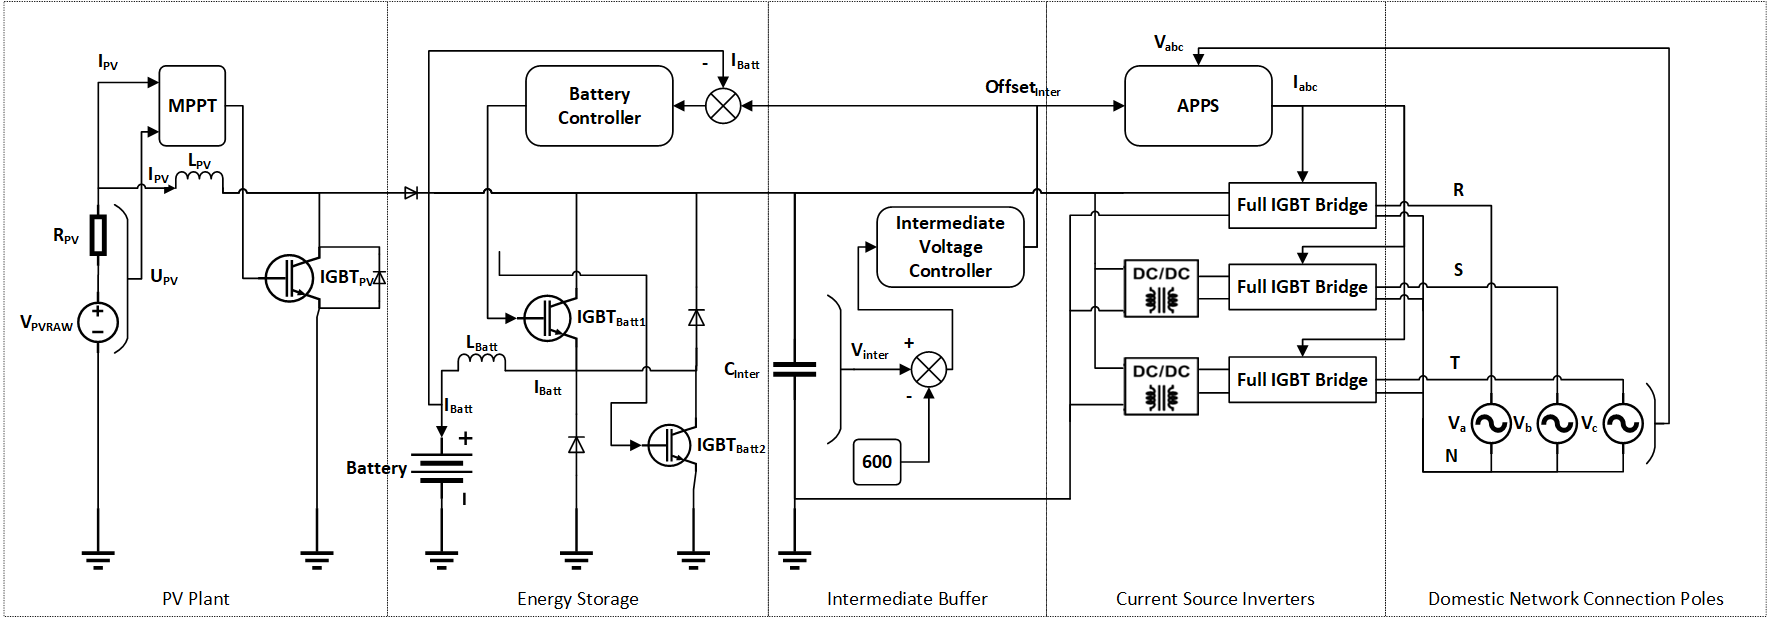
\includegraphics[width=1.5\textwidth,angle=-90]{Unblance_EPS_Pics/PowerTopology_full.png}
        \caption{Full topology of the VU compensator. The device is segmented into PV plant as a renewable energy source with added MPPT unit, power storage with a Li-ion battery extended with charger/discharge half bridge, buffer capacitance with intermediate voltage controller, three separated CSI with DC-DC isolators, and the network substituting voltage sources.}
        %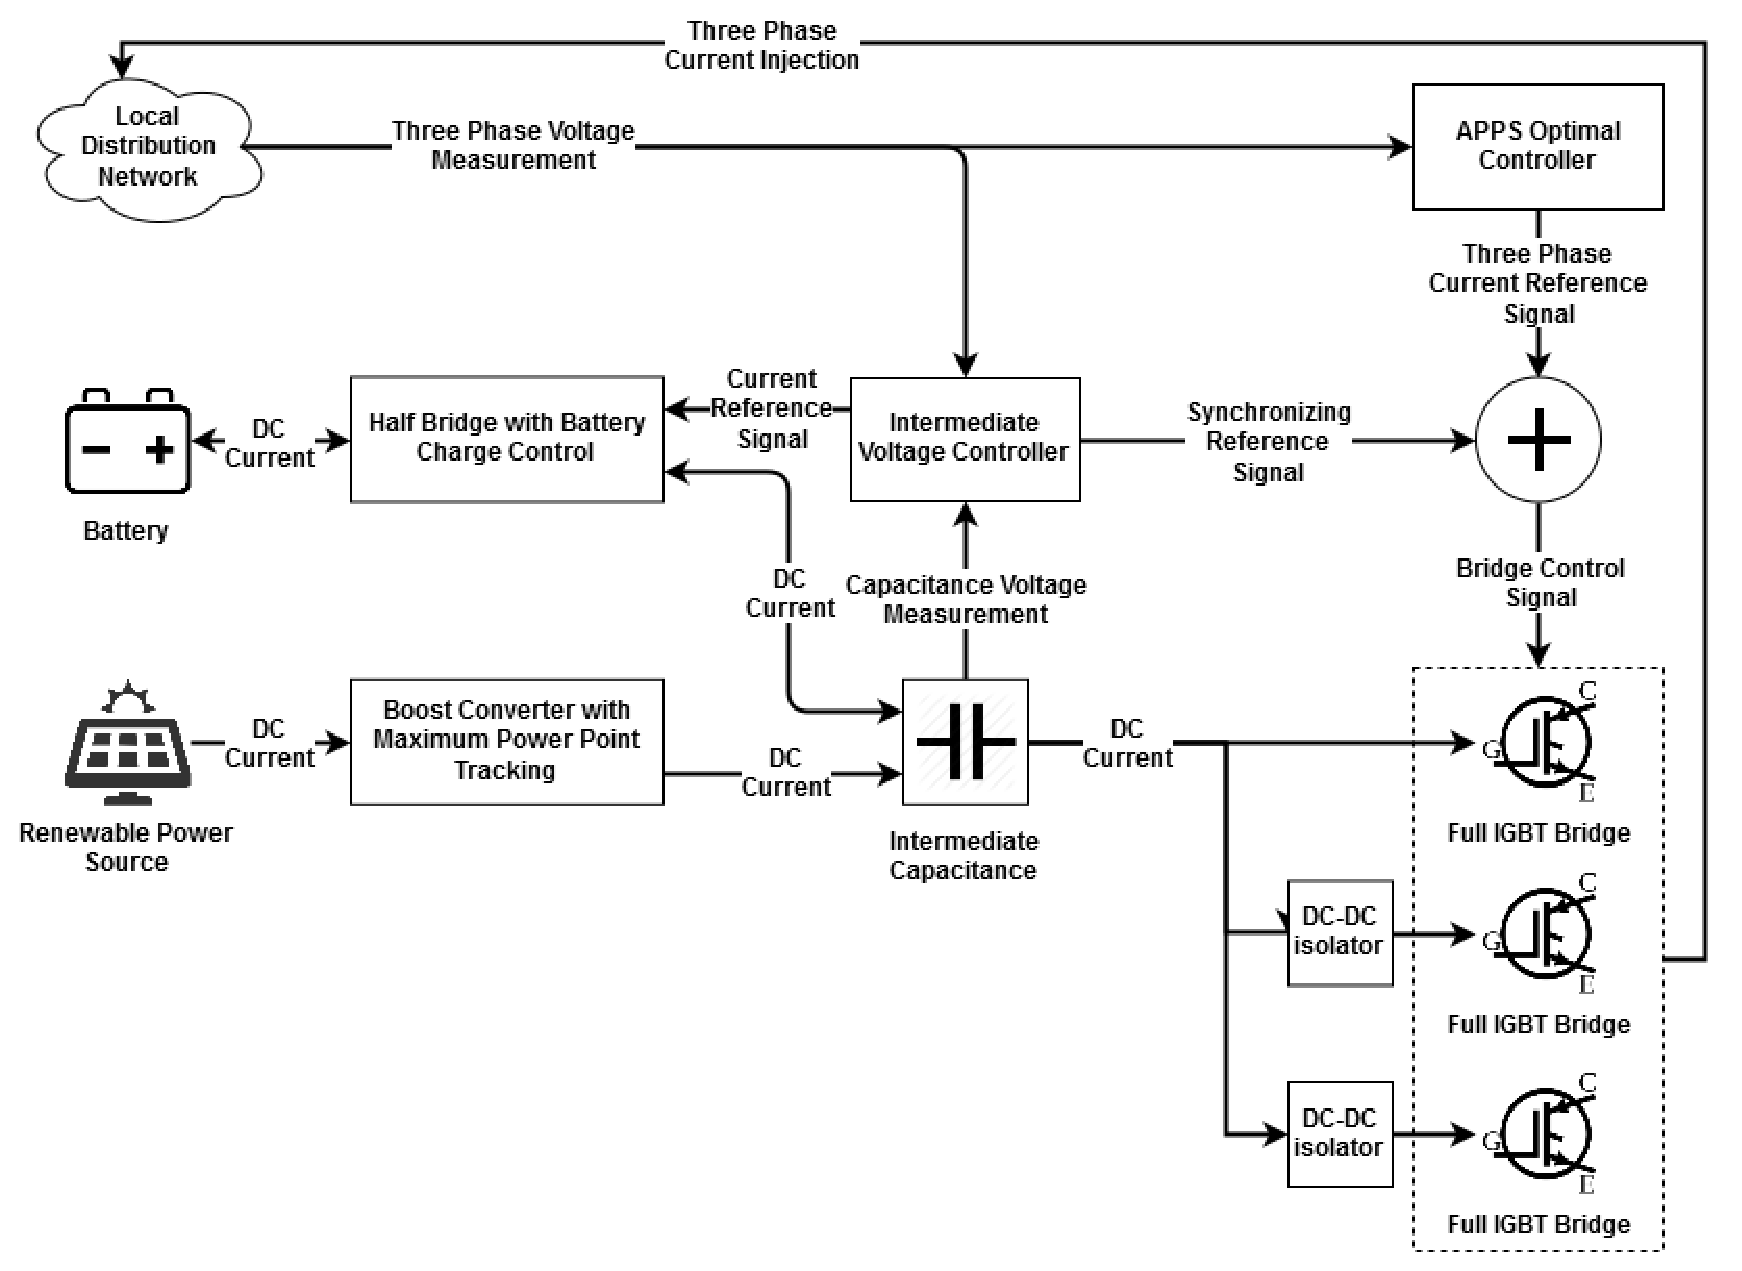
\includegraphics[width=0.95\textwidth]{Unblance_EPS_Pics/inverter.eps}
%        \caption{The asymmetrical inverter design, which applies three single phase full bridge IGBT current injector to create the injected asymmetrical current shapes for voltage unbalance compensation.}
        \label{fig:inv}
        \end{figure*}

        Of course there is a possibility that there is no renewable power available for a longer period of time and the battery completely looses its charge. In this case the system should work merely with the power of the connection point but with zero energy balance. This states to operate two controller with semi-opposite control goals. The optimization based controller requires current injection while the intermediate voltage controller (Figure \ref{fig:inv}) keeps the inverters energy balance. Although for this operation some of the control's performance should be sacrificed, unbalance compensation could be achieved even without external renewable power, and energy storage at a minimum power requirement. The individual physical values of the CSI can be observed in Table \ref{tbl:params}.\\

        \begin{table}[]
    \center
		\caption{The applied parameters and physical values in the VU compensator design}
        \begin{tabular}{|l|l|}
        \hline
        Parameter      & Value  \\ \hline
        $R_{PV}$     & 5 $\Omega$ \\ \hline
        $L_{PV}$ & 100 $mH$\\ \hline
        $L_{Batt}$ & 100 $mH$\\ \hline
        $L_{CSI}$ & 2 $mH$\\ \hline
        $C_{inter}$ & 10 $mF$\\ \hline
        $V_{Batt}$ & 153.6 $V$\\ \hline
        $\widehat{V}_{PV}$ & 30 $V$\\ \hline
        $C_{Batt}$ & 200 $Ah$\\ \hline
        $K_{P}$ & 1 \\ \hline
        $K_{D}$ & 0.8\\ \hline
        $p_{inter}$ & 200\\ \hline
        \end{tabular}
        \label{tbl:params}
    \end{table}

        In the following paragraphs the sub-stages of the VU compensating device shall be explained in detail, and they role in solving the control problem.}

        \subsubsection{\hlc[PT]{PV energy source}}
        The PV plant is the renewable power source of the device, modelled as a controlled voltage source with the value of $V_{PV}$, and with serial resistance $R_{PV}$, and filtering inductance of $L_{PV}$. The voltage source was modelled with periodic pattern, as PV panels give variable power output as well. For continuous operation a maximum power point tracker (MPPT) was implemented as this is the state of the art handling of uncertain PV sources as suggested in \cite{ali2012survey}. The MPPT controls a single IGBT of which emitter leg is connected to the ground.

        \subsubsection{\hlc[PT]{Energy storage}}
        A Li-ion battery with 153.6 V and 200 Ah, with series choke inductance of $L_{Batt}$ is providing energy storage capability, when the PV source is not present, or the required mitigation is too low to dissipate all the energy to the network. For controlling the power flow, a classic half-bridge structure was employed, with a simple windowed control with 10 kHz switching frequency. The reference signal is set by the battery's current $I_{Batt}$ subtracted from the intermediate voltage controller's reference $Offset_{inter}$.

        \subsubsection{\hlc[PT]{Intermediate buffer}}

        The in intermediate buffer capacitance was placed between the energy storage stage and the CSI actuators. This stage is responsible for the whole device's energy management, via an intermediate voltage control scheme. The intermediate voltage controller's flowchart can be observed on Fig.\ref{fig:interV}, where $K_P$, $K_D$ are the controller gains, and $p_{inter}$ is the filter's gain. The $Offset_{inter}$ signal is responsible, to hinder the APPS by lowering the gain value of compensation as seen in algorithm \ref{algo:APPS}. Furthermore, to direct the power flow from the battery into the intermediate buffer capacitance, via the battery controller's reference signal.

        \begin{figure}[t]
        \centering
        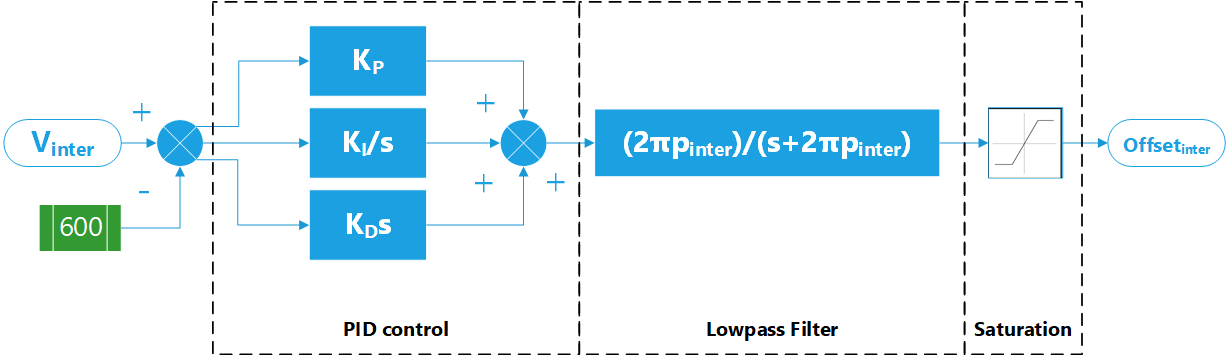
\includegraphics[width=\textwidth]{Unblance_EPS_Pics/Intermediate.png}
        \caption{A general PD scheme and low pass filter of the intermediate voltage controller.}
        \label{fig:interV}
        \end{figure}

        \subsubsection{\hlc[PT]{Current source inverters and dynamic network}}

        To be able to facilitate the harmonic currents the APPS generates as output, an unbalanced inverter structure was employed. The most straight forward way to implement such a design, is to use three galvanically decoupled one phase CSIs. The decoupling was described in section \oldref{BASICCSR:sec:DCDC}, and the single phase design in section \oldref{BASICCSR:sec:CSI}, although only one choke inductance ($L_{CSI}$) was used per phase.\\



    \section{Discussion}\label{VUB:sec:Discussion}

%write stuff here..

    \subsection{Dynamical simulation based experiments}\label{VUB:sec:Results}
		
    In order to be able to investigate the proposed optimization based unbalance reduction control structure with the three phase inverter on a low voltage local grid, all the elements of this complex electrical system (including the photovoltaic source, the inverter, the battery and the nonlinear local grid with different types of loads) has been modeled in Matlab/Simulink environment. The primary aim of the simulation based experiments were to serve as a proof of concept for the proposed complex control structure.

    \subsection{Performance analysis}\label{VUB:sec:Performance}

    The aim of performance analysis is twofold. First of all, the proposed voltage unbalance indicator has to be investigated in the control structure as the cost function of the optimization based controller, and on the other hand, the control structure itself has to be exposed against engineering expectations.


            The results of the first experiment can be seen in Figure \ref{fig:compare_asym_PV} where the geometrical norm \ref{equ:geom} has been used as the voltage unbalance indicator and the cost function for the optimizer.  The dashed line represents the examined low voltage local network's unbalance norm ($G$) without the proposed controller implemented in the inverter unit of the domestic powerplant while the solid line represents the compensated network's norm value. The performance of the controller with this norm is apparent, it was able to decrease the network voltage unbalance by approximately 85 \%. In this experimental setup the controller has enough input energy due to the batteries and the available solar power.

            \begin{figure*}[ht]
            \centering
            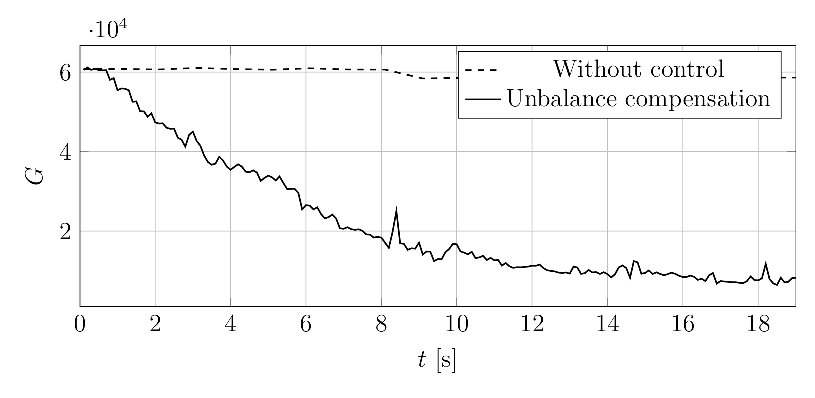
\includegraphics[width=0.95\textwidth]{Unblance_EPS_Pics/UnbalRedComp_JCP-figure3.eps}
            \caption{Unbalance reduction control system performance with half charged battery and photovoltaic power source available. The underlying unbalance norm is the geometrical one ($G$) in this experiment. After starting the controller at $t=0.1s$ the unbalance measure $G$ of the network significantly decrease.}
            \label{fig:compare_asym_PV}
            \end{figure*}

            \begin{figure*}[ht]
            \centering
            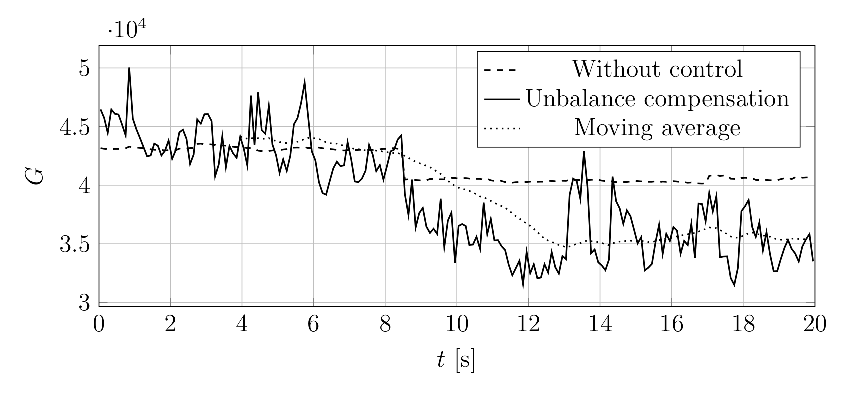
\includegraphics[width=0.95\textwidth]{Unblance_EPS_Pics/UnbalRedComp_JCP-figure4.eps}
            \caption{Unbalance reduction control system performance without battery and renewable source (zero energy balance operation). The performance reduction is clearly observable compared to the case when external power source is available (Figure \ref{fig:compare_asym_PV}), but as result the voltage unbalance indicator $G$ reduced by the average value of 14.78\%.}
            \label{fig:compare_asym}
            \end{figure*}

            A slightly more challenging situation is investigated in Figure \ref{fig:compare_asym} where the controller had had to operate without photovoltaic source and batteries. This is called zero moving average balance operation mode when the energy obtained from the network is re-injected in such a way that the unbalance indicators decrease. It can be seen that the performance of the controller is modest than that of Figure \ref{fig:compare_asym_PV}, but it is still acceptable.

      \subsubsection{Robustness analysis}\label{VUB:sec:Robustness}

            The robustness of the proposed control structure is an important qualitative property with respect to the time dependent loads present on the network. The robustness of the proposed controller had to be tested via simulation when different types of loads (inductive, capacitive, resistive) had been varied in step changes representing the on/off switching the different types of household appliances (motors, switching mode power supplies, electric heaters, etc.). In the experiment depicted in Figure \ref{fig:robustness}, a load change has been introduced to the network in every 15 seconds causing the voltage unbalance to jump to a different value (measured in the geometrical norm \ref{equ:geom}). As it can be seen in the figure the controller successfully compensates the unbalance after each transient.

              \begin{figure*}[ht]
            \centering
            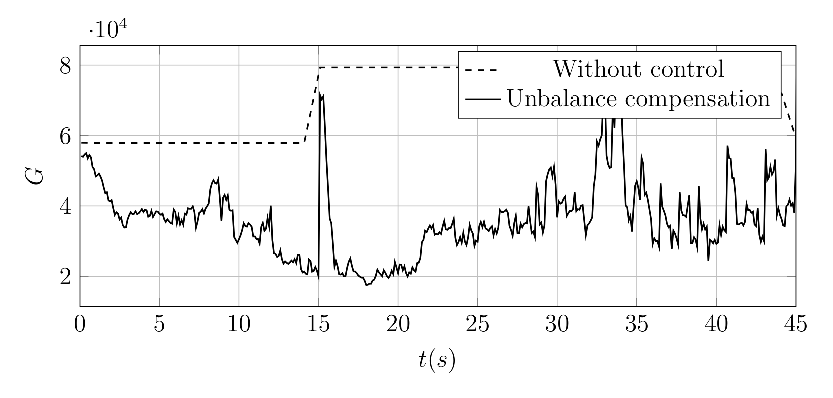
\includegraphics[width=0.95\textwidth]{Unblance_EPS_Pics/UnbalRedComp_JCP-figure5.eps}
            \caption{Robustness analysis with respect to step type changes in the network load (and voltage unbalance). The unbalance reduction controller successfully compensates the changes in the network voltage unbalance norm ($G$) value.}
            \label{fig:robustness}
            \end{figure*}

            \subsubsection{Measurements from a real unbalanced network}\label{VUB:sec:Measurement}

            The measurements took place at the campus building's power electronics laboratory, where a common 400\,V connection point was investigated as the behaviour of the network. The three phase 230\,V line-to-ground voltages has been transformed to 6\,V to be effectively measurable in time domain with high performance NI-USB DAQ on 10\,ksample/s. Because of the limited computational capacity only a 10 second measurement was made in every hour.  The measurements then has been merged and smoothed to eliminate the inter-measurement transients.\\
            Afterwards, the measurement data has been used as the input of a micro-grid segment of the Matlab/Simulink model, to test the controller and inverters structure's performance in quasi-realistic circumstances. The controllers performance on the simulated microgrid's network loss reduction can be observed on Figure \ref{fig:compare_power} and Figure \ref{fig:u_inter}. The measurement output is connected to a modeled three phase load and network system, consisting of symmetrical loads and network segments between them. Further artificial load unbalance is not necessary since the network's unbalance is already present. This structure enables to show that any point the inverter is connected, could restore power quality with a certain degree such unbalance compensation at this case. The future plan is to set up multiple devices on different connection points.

    \subsection{Environmental effect}\label{VUB:sec:Environment}

    The favorable effects of the proposed unbalance reduction control algorithm , i.e. increase power quality not only at the connection point but in the whole low voltage transformer area, which causes a reduction of the effective power loss and the reduction in the CO${}_2$ emission.

        \subsubsection{Power loss reduction on the network}\label{VUB:sec:Powerloss}

             Network loss reduction due to the unbalance reduction compensation control is investigated on Figure \ref{fig:compare_power} where the simulation experiment was carried out in the circumstance when the renewable source was not shut down (e.g. insufficient amount of sunlight) and additionally the battery was drained completely  \cite{Neukirchner2015}, \cite{neukirchner2015examination}.

            \begin{figure*}[ht]
            \centering
            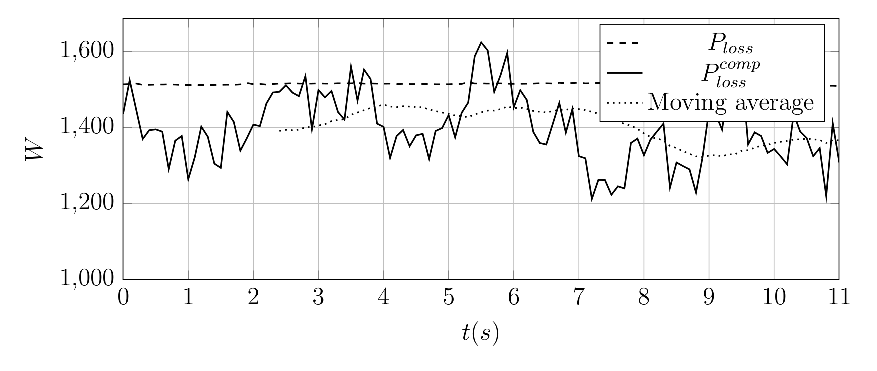
\includegraphics[width=0.95\textwidth]{Unblance_EPS_Pics/UnbalRedComp_JCP-figure6.eps}
            \caption{Compensation control's loss reduction during zero energy balance operation on the modeled network, where $P_{loss}$ indicates the effective power losses and $P^{comp}_{loss}$ effective power losses during control of the network. As result the network losses reduced by mean $6.5\%$.}
            \label{fig:compare_power}
            \end{figure*}

            The results show that despite of the negative cross effects of the intermediate voltage controller and the unbalance reduction controller it was possible to find the trade-off between the control goals of the different controllers (maintain zero energy balance for the inverter and decrease the unbalance on the network). The estimated loss reduction in the experimental setup is 6.5\%.

            \begin{figure*}[ht]
            \centering
            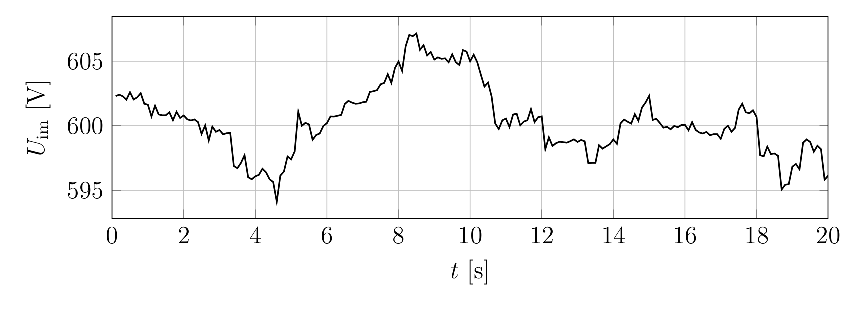
\includegraphics[width=0.95\textwidth]{Unblance_EPS_Pics/UnbalRedComp_JCP-figure7.eps}
%                  %\pgfplotsset{every tick label/.append style={font=\tiny},legend style={at={(1,1)},anchor=north east}}
%                 \pgfplotsset{every tick label/.append style={font=\normalsize}}
%                 \begin{tikzpicture}
%                 \begin{axis}[
%                     width=\textwidth,
%                     height=5cm,
%                     xlabel = {$t$~[s]},
%                     ylabel = {$U_{\textnormal{im}}$~[V]},
%                     grid=major,
%                     xmin=0,
%                     xmax=20,
%                     %ymin=0,
%                     ]
%                     \addplot[thick] table {netw_plot/U_inter.dat};
%                     %\legend{\scriptsize$U_{intermediate}$}
%                     \end{axis}
%                  \end{tikzpicture}
                 \caption{Intermediate puffer capacitance's voltage within boundaries ($600\pm10$\,V), during zero energy balance operation mode of the voltage unbalance compensation controller. $U_{\textnormal{im}}$ indicates intermediate the capacitance's voltage.}
                 \label{fig:u_inter}
                \end{figure*}

%        \subsubsection{Malfunction rejection}
%
%            asd

        \subsubsection[CO2 footprint]{CO$_2$ footprint}\label{VUB:sec:CO2}

            The fact that this controller enables the reactive power reduction has a favourable consequence, i.e. the power loss or equivalently CO$_2$ emission and the carbon footprint can also be decreased. The estimated environmental effects of voltage asymmetry compensation can be calculated. Let us assume 3000\,kWh for the yearly electric energy consumption an average household and $9.173\%$ for the loss of the distribution network at 2013 \cite{MVM2013} and $7.654\%$ at 2018 \cite{MVM2018}. Using the controller the losses on the simulated network are reduced by 6.5\%. The calculation follows \ref{eqn:co_emission}:

            \begin{equation}
                \label{eqn:co_emission}
                \begin{array}{rcl}
                 P_{loss}&=&3000\,\textnormal{kWh}\cdot7.654\%\\
                P^{comp}_{loss}&=&3000\,\textnormal{kWh}\cdot(7.654\cdot0.93)\%\\
                 \Delta P_{loss}&=&P_{loss}-P^{comp}_{loss}\\
                 \end{array}
                \end{equation}

            where $P_{loss}$ is the assumed network loss per household and $P^{comp}_{loss}$ is s the assumed network loss with unbalance compensation control and $\Delta P_{loss}$ is the saved energy. According to \ref{eqn:co_emission}, unbalance compensation results in an energy savings of 19.26 kWh in 2013 and 16.07 kWh in 2018. Taking into account the proportion of power currently generated by fossil fuels (coal 17.3\%, gas 38.3\% at 2013 \cite{MVM2013}, \cite{gorbe2012reduction} and coal 13.1\%, gas 51.4\% at 2018 \cite{MVM2018}) and the rate of $\textnormal{CO}_2$ emission during electric energy production (1,000\,g/kWh from coal and 430\,g/kWh from gas), it can be concluded that voltage unbalance compensation could reduce $\textnormal{CO}_2$ emissions by 6504.9\,g a year in 2013 and 5656.96\,g in 2018 in an average household. Note that this result reflect only the proof of concept, due the neglected power losses of the inverter and the artificial load of the network.
						
						%2105.17+3551.79

\section{Conclusion}\label{VUB:sec:Conclusion}

    Currently used measures of voltage unbalance (see section \oldref{BASICUNB:sec:DefinitionsofUNB}) has been extended in this chapter with a new norm candidate, namely a geometrical norm, where the magnitude of voltage unbalance are evaluated by the symmetrical difference of the voltage phasor triangles. It is more demanding from the computational point, of view but has an interesting feature namely it checks electrical asymmetry, i.e. the norm of a $\pm120$ degree  rotated version of the ideal three-phase phasor is zero in the geometrical sense.\\
    This way, the defined norm is applied as a cost function in the asymmetry reducing controller structure utilizing an asynchronous parallel pattern search (APPS) algorithm also presented in the thesis. Simulations, performed in Matlab/Simulink environment show that the geometrical based indicator can serve as a basis of further research. The suggested controller structure enables the residential users owning a grid synchronized domestic power (renewable) plant to reduce voltage unbalance measurable at the connection point. The fundamental element of the system is a modified three phase inverter that is capable of the asymmetric current injection of any current waveforms to the network, via decoupled bi-directional DC-DC converters. The optimization-based control algorithm injects the available energy (as current waveform) in such a way, that the voltage unbalance decreases. This is an optimization problem which is constrained by the available renewable energy supplied by the power plant, or energy storage unit.\\
    The control structure has been tested on a low voltage network model in a dynamical simulation environment consisting of the models of the electrical grid, a domestic power plant, an asymmetrical inverter circuit, and different types of loads. Different simulation experiments has been run for each norm and for both the power constrained and unconstrained case. The preliminary results show that this structure can serve as a residential level voltage quality improvement method for the three phase low voltage network also indirectly reduces the CO${}_2$ emission due facilitating more effective energy usage.

%\section{Voltage unbalance compensation with optimization based control algorithm and asymmetrical inverter structure}
%
%    Based on the proposed measures of voltage unbalance it is possible to formulate some power quality related aims, or demands for the domestic size generator units as follows.
%
%    \subsection{Problem statement}
%
%    The voltage and current unbalance presents in the three phase low voltage transformer area causes additional power loss inside the medium voltage/low voltage transformer and in the transportation line wires too. It also has undesired effects in certain three phase loads, mainly rotating machines where it causes torque reduction and pulsating torque effect. Large scale unbalance can activate automatic protection functions of electricity dispatch system causes power outage. This is unpleasant for the customers and adds maintenance cost to the service provider. These negative effects lower the electric power quality and rises the cost of electrical energy and rises the carbon footprint of our everyday life. Our aim to develop a three phase instrumentation, which can compensate these undesirable effects, lower or eliminate the voltage and current unbalance to lower the power losses and the CO${}_2$ emission and increase power quality not only at the connection point but in the whole low voltage transformer area. \emph{It is important to note, that this power quality improvement can be achieved without any significant added cost.} The aim is to integrate this function into an existing three phase photovoltaic inverter device connected to the low voltage grid, and the created complex energetic system is able to inject the renewable energy to the transportation network, can store the electrical energy from stochastic renewable sources in electrical vehicle batteries or feed the grid from the charged batteries in energy deficit and high demand simultaneous situations. Our new added value the integrated control algorithm which can highly lower or eliminate the observed unbalance of the network.
%
%    \subsection{Control problem}
%
%    The above problem statement partially specifies the solution space together with the solution method. The system of interest is the power grid with all the stochastic and nonlinear phenomena present in it. The input to the system is the current signals (one current in the single phase case and three in the three phase setup), which are naturally constrained by the available energy of the household - stored in a battery pack or momentarily generated by the wind or solar generator unit. The response of the system can be either the current or the voltage measured at the connection point of the inverter unit, however, the general legal regulations only allow voltage measurement for consumers. The difficulty of the control problem comes from the fact, that there are no mathematically tractable models of the network can be generated because of its unpredictable and nonlinear features. This means, that only black-box methods can be applied for this system.
%
%    For the control aim it is a natural choice to minimize the actual voltage unbalance of the low voltage local transformer area measured (or calculated) at the connection point of the inverter. Several optimization based methods are available for such kind of optimal control problems, e.g.  \cite{gorbe2012reduction} where the only bottleneck is the computational efficiency since the impemented controller has to run on the commercial inverter's hardware (digital singal processor unit).
%
%    \subsection{Asymmetrical inverter structure}
%
%    \textcolor{blue}{
%        The renewable energy injection is realized increasingly directly to the three phase low voltage grid in domestic size photovoltaic power plants too. This can reduce the voltage and current unbalance caused by the stochastic power production of wind and solar sources. More and more manufacturers produce three phase grid synchronized inverters from 5\,kW size. These equipments implement accurate symmetrical current feed with a standard three phase full bridge structure consists of six Isolated Gate Bipolar Transistors (IGBT). This is a cost effective standard structure suitable for symmetric harmonic current injection. It has limited capacities to inject not totally symmetric 3 phase current time functions, but Kirchhoff's current law permits only constant zero-sum current time functions injected with this structure. There are examples with this type of asymmetric current injections in the literature \cite{lee2010new}.}
%
%         %ide kellene a hivatkozás arra a cikkre, amit mutattál, ahol nem 120 fokosak a vektorok a fazor diagrammon, de az összegük 0
%    \textcolor{blue}{
%        This type of current injections has limited compensation capacity and this is not enough in  most asymmetric production and load cases. In our case we need more general, not specific asymmetric current waveforms, because the proposed control aim assumes the ability of injecting non zero-sum currents. This needs special inverter design structure. We need zero line connection for the differential current. One of the possible solution is to use 3 different full bridge single phase current inverters to supply each phase of low voltage transportation lines \cite{Patnaik2013topologies}. But in this case we need galvanic isolations of these single phase inverters in the output, or in the DC input size.}
%
%        %ide tegyük be hivatkozásnak: "Sushree Sangita Patnaik ., Anup Kumar Panda:Three-level H-bridge and three H-bridges-based three-phase four-wire shunt active power filter topologies for high voltage applications"
%    \textcolor{blue}{
%        This isolation can be reached  with using isolation transformers in the supply side. But we would like to use it a complex energetic system with specific inside true DC bus system feeded from Photovoltaic panel or batteries. We have to isolate  at least 2 full bridges with two way DC-DC converters. This can complicate the physical realization but easy to simulate with two controlled power source. Other possible easy to realize solution to isolate the full bridge outputs  connected to three phase lines with isolating transformers. It is recommended for operating and electric shock protection reasons too (Figure \ref{fig:asymminvwithgalvanic transformer}).Our distant aim to compensate other operational type line failures, such zero current appearing. This isolation method doesn't allow to produce CD current components, thats why we are looking for other design. Possible elegant solution to supplement the standard three phase inverter design with a fourth half bridge for Zero line, building a specific four leg inverter design \cite{Ninad2014control}.}
%
%        %ide tegyük be hivatkozásnak: "Nayeem Ahmed Ninad ., Luiz Lopes:Per-phase vector control strategy for a four-leg voltage source inverter operating with highly unbalanced loads in stand-alone hybrid systems"
%    \textcolor{blue}{
%        Only drawback of this solution is the complex difficult control method of the half bridges, to keep the current sum in zero values in each moment, and to provide the correct current paths inside the inverter. This structure has the lowest production cost, but in the phase of proofing the asymmetry compensation we chose the DC-DC isolated  full bridge design for simulation purpose because of the simple control during simulation.}
%    \textcolor{blue}{
%        As a further generalization step, the injection of no harmonic current shapes will be necessary in order to decrease the extant Total Harmonic Distortion (THD) of the network. These expectations yield an inverter with new structure suitable for arbitrary current injections without limitations. The design lends similar elements like in \cite{gorbe2012reduction} by means of battery charge, renewable power point tracking, intermediate voltage, and IGBT bridge control, but in this case the problem requires a three phase solution for the voltage unbalance reduction. The applied structure based on a full bridge IGBT structure used in single phase current injection. Three different IGBT full bridge were connected at the output point, thus our structure has three phase and neutral connection too, to carry out any current form. The disadvantage of this structure is that it needs 12 IGBTs in the output stage as opposed to the 6 IGBTs needed for a classical full bridge structure and needs three galvanically isolated direct current (DC) voltage source for feeding.}
%    \textcolor{blue}{The other standard elements, that the inverter design consists:}
%
%
%
%        \begin{itemize}
%            \item\textcolor{blue}{ Standard maximum power point tracking (MPPT) input stage, to inject the maximum available power from the renewable source to the intermediate voltage capacitor with a simple controlled boost converter}
%            \item\textcolor{blue}{ A half bridge current controller to charge or deploy the battery pack connected to the complex energetic system for energy storage and energy unbalance compensation}
%            \item\textcolor{blue}{ Intermediate voltage controller}
%            \item\textcolor{blue}{ Universal three phase output stage with 3 single phase full bridge IGBT current injector and 2 high current DC-DC converter}
%        \end{itemize}
%    \textcolor{blue}{
%        This is suitable to inject any necessary current shape to the low voltage three phase grid connection even DC currents too. Later a power loss and production cost analysis will be necessary if the built structure will be suitable for asymmetric compensation of low voltage transformer area.}
%
%        %\begin{figure*}[ht]
%%            \centering
%%            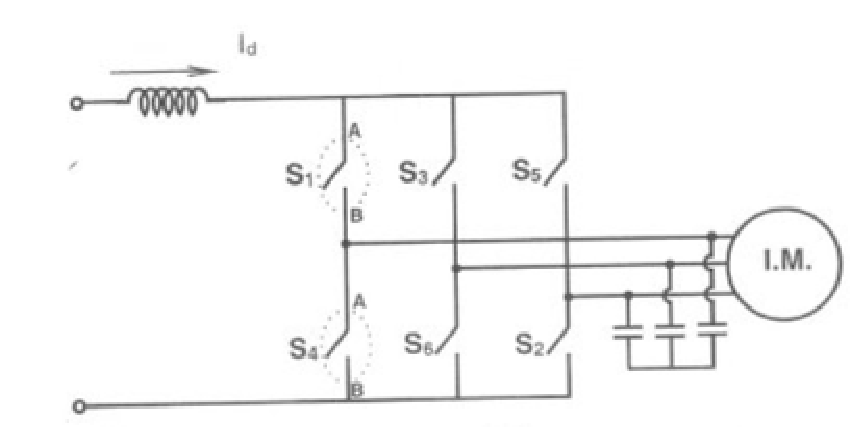
\includegraphics[width=0.95\textwidth]{standard_inverter.eps}
%%            \caption{\textcolor{blue}{Standard symmetrical current inverter design, implies 6 IGBT current injector with serial inductance. }}
%%        \label{fig: symminv}
%%        \end{figure*}
%
%        %\begin{figure*}[ht]
%%            \centering
%%            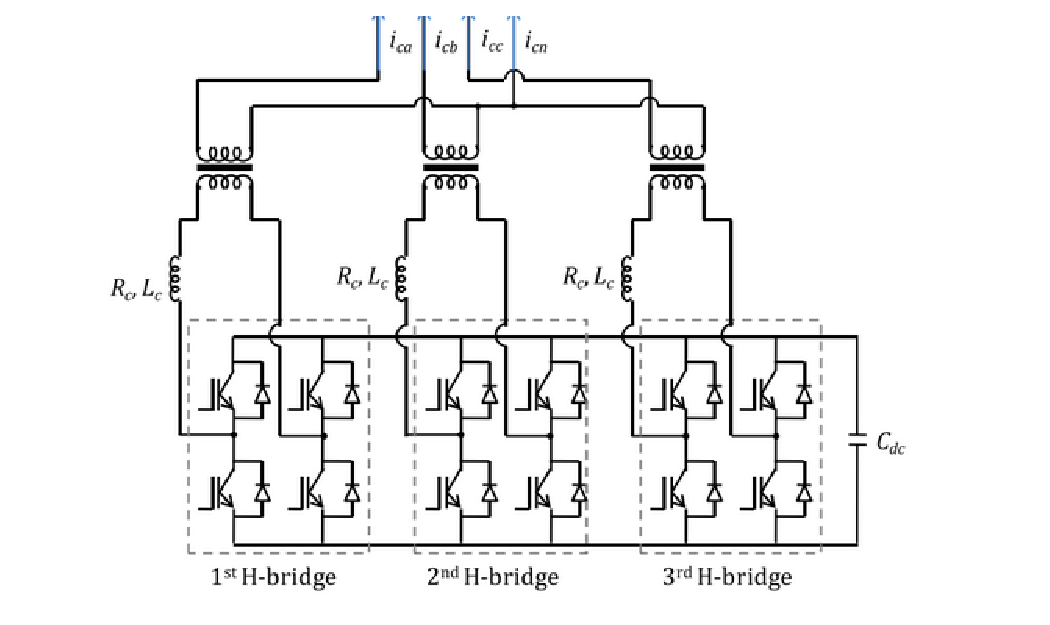
\includegraphics[width=0.95\textwidth]{isolated_inverter.eps}
%%            \caption{\textcolor{blue}{Asymmetrical inverter design with three separated H-bridges.}}
%%        \label{fig: asymminvwithDCgalvanic transformer}
%%        \end{figure*}
%
%\begin{figure}[h]
%          \begin{center}
%                \begin{circuitikz}[scale=.5, european] %% => Itt ne állíts a skálát, inkább a figure-nél!%%
%                %\draw[help lines] (0,0) grid (16,40);
%
%                \draw%[color=magenta]
%                    %% híd
%                    (0,0) to[C=$C_{intermediate}$] (0,38)
%                    (0,0) to[short] (10,0)
%                    (6,0) node[nigbt, anchor=E](nigbt33){}
%                    (nigbt33.E) node[circ]{}
%
%                    (10,8) node[nigbt, anchor=E,xscale=-1](nigbt32){}
%
%                    (6,8) node[nigbt, anchor=E](nigbt31){}
%                    (nigbt33.C) to[short] (nigbt31.E)
%
%                    (10,0) node[nigbt, anchor=E, xscale=-1](nigbt34){}
%                    (nigbt34.C) to[short] (nigbt32.E)
%
%                    (nigbt32.C) to[short] (10,12)
%                    (nigbt31.C) to[short,-*] (6,12)
%                    (4,12) to[short] (10,12)
%                    (4,12) to[short,-*] (4,38)
%
%
%                    %%trafó
%                    (7,6) node[transformer,rotate=90,transform shape,american](T3){}
%                    (T3.B1) to[short,-*] (6,7.05)
%                    (T3.B2) to[short,-*] (10,7.05)
%                    (T3.A1) to[short] (7,4)
%                    (7,4) to[short,-o] (13,4) node[anchor=west] {$N$}
%                    (T3.A2) to[short,-o] (13,4.95) node[anchor=west] {$T$}
%                    ;
%
%                    \draw%[color=blue]
%                    %% híd
%                    (3,13) to[short,*-] (10,13)
%                    (6,13) node[nigbt, anchor=E](nigbt23){}
%                    (nigbt23.E) node[circ]{}
%
%                    (10,21) node[nigbt, anchor=E,xscale=-1](nigbt22){}
%
%                    (6,21) node[nigbt, anchor=E](nigbt21){}
%                    (nigbt23.C) to[short] (nigbt21.E)
%
%                    (10,13) node[nigbt, anchor=E, xscale=-1](nigbt24){}
%                    (nigbt24.C) to[short] (nigbt22.E)
%
%                    (nigbt22.C) to[short] (10,25)
%                    (nigbt21.C) to[short,-*] (6,25)
%                    (4,25) to[short,*-] (10,25)
%
%
%
%
%                    %%trafó
%                    (7,19) node[transformer,rotate=90,transform shape,american](T2){}
%                    (T2.B1) to[short,-*] (6,20.05)
%                    (T2.B2) to[short,-*] (10,20.05)
%                    (T2.A1) to[short] (7,17)
%                    (7,17) to[short,-*] (12,17)
%                    (T2.A2) to[short,-o] (13,17.95) node[anchor=west] {$S$}
%                    ;
%
%                    \draw%[color=cyan]
%                    %% híd
%                    (3,26) to[short] (10,26)
%                    (3,26) to[short,-*] (3,0)
%
%                    (6,26) node[nigbt, anchor=E](nigbt13){}
%                    (nigbt13.E) node[circ]{}
%
%                    (10,34) node[nigbt, anchor=E,xscale=-1](nigbt12){}
%
%                    (6,34) node[nigbt, anchor=E](nigbt11){}
%                    (nigbt13.C) to[short] (nigbt11.E)
%
%                    (10,26) node[nigbt, anchor=E, xscale=-1](nigbt14){}
%                    (nigbt14.C) to[short] (nigbt12.E)
%
%                    (nigbt12.C) to[short] (10,38)
%                    (nigbt11.C) to[short,-*] (6,38)
%                    (0,38) to[short] (10,38)
%
%
%                    %%trafó
%                    (7,32) node[transformer,rotate=90,transform shape,american](T1){}
%                    (T1.B1) to[short,-*] (6,33.05)
%                    (T1.B2) to[short,-*] (10,33.05)
%                    (T1.A1) to[short] (7,30)
%                    (7,30) to[short] (12,30)
%                    (12,30) to[short,-*] (12,4)
%                    (T1.A2) to[short,-o] (13,30.95) node[anchor=west] {$R$}
%                    ;
%                %%
%                \end{circuitikz}
%                \caption{\textcolor{blue}{Simplified asymmetrical inverter design employing three galvanically isolated H-bridges with transformers for DC-DC isolation substitution.}}
%                \label{fig: asymminvwithgalvanic transformer}
%          \end{center}
%    \end{figure}
%
%        %\begin{figure*}[ht]
%%            \centering
%%            \includegraphics[width=0.95\textwidth]{isolated_only_inverter.eps}
%%            \caption{\textcolor{blue}{Simplified asymmetrical inverter design employing three galvanically isolated H-bridges with transformers for DC-DC isolation substitution.}}
%%        \label{fig: asymminvwithgalvanic transformer}
%%        \end{figure*}
%
%
%        \begin{figure*}[ht]
%        \centering
%        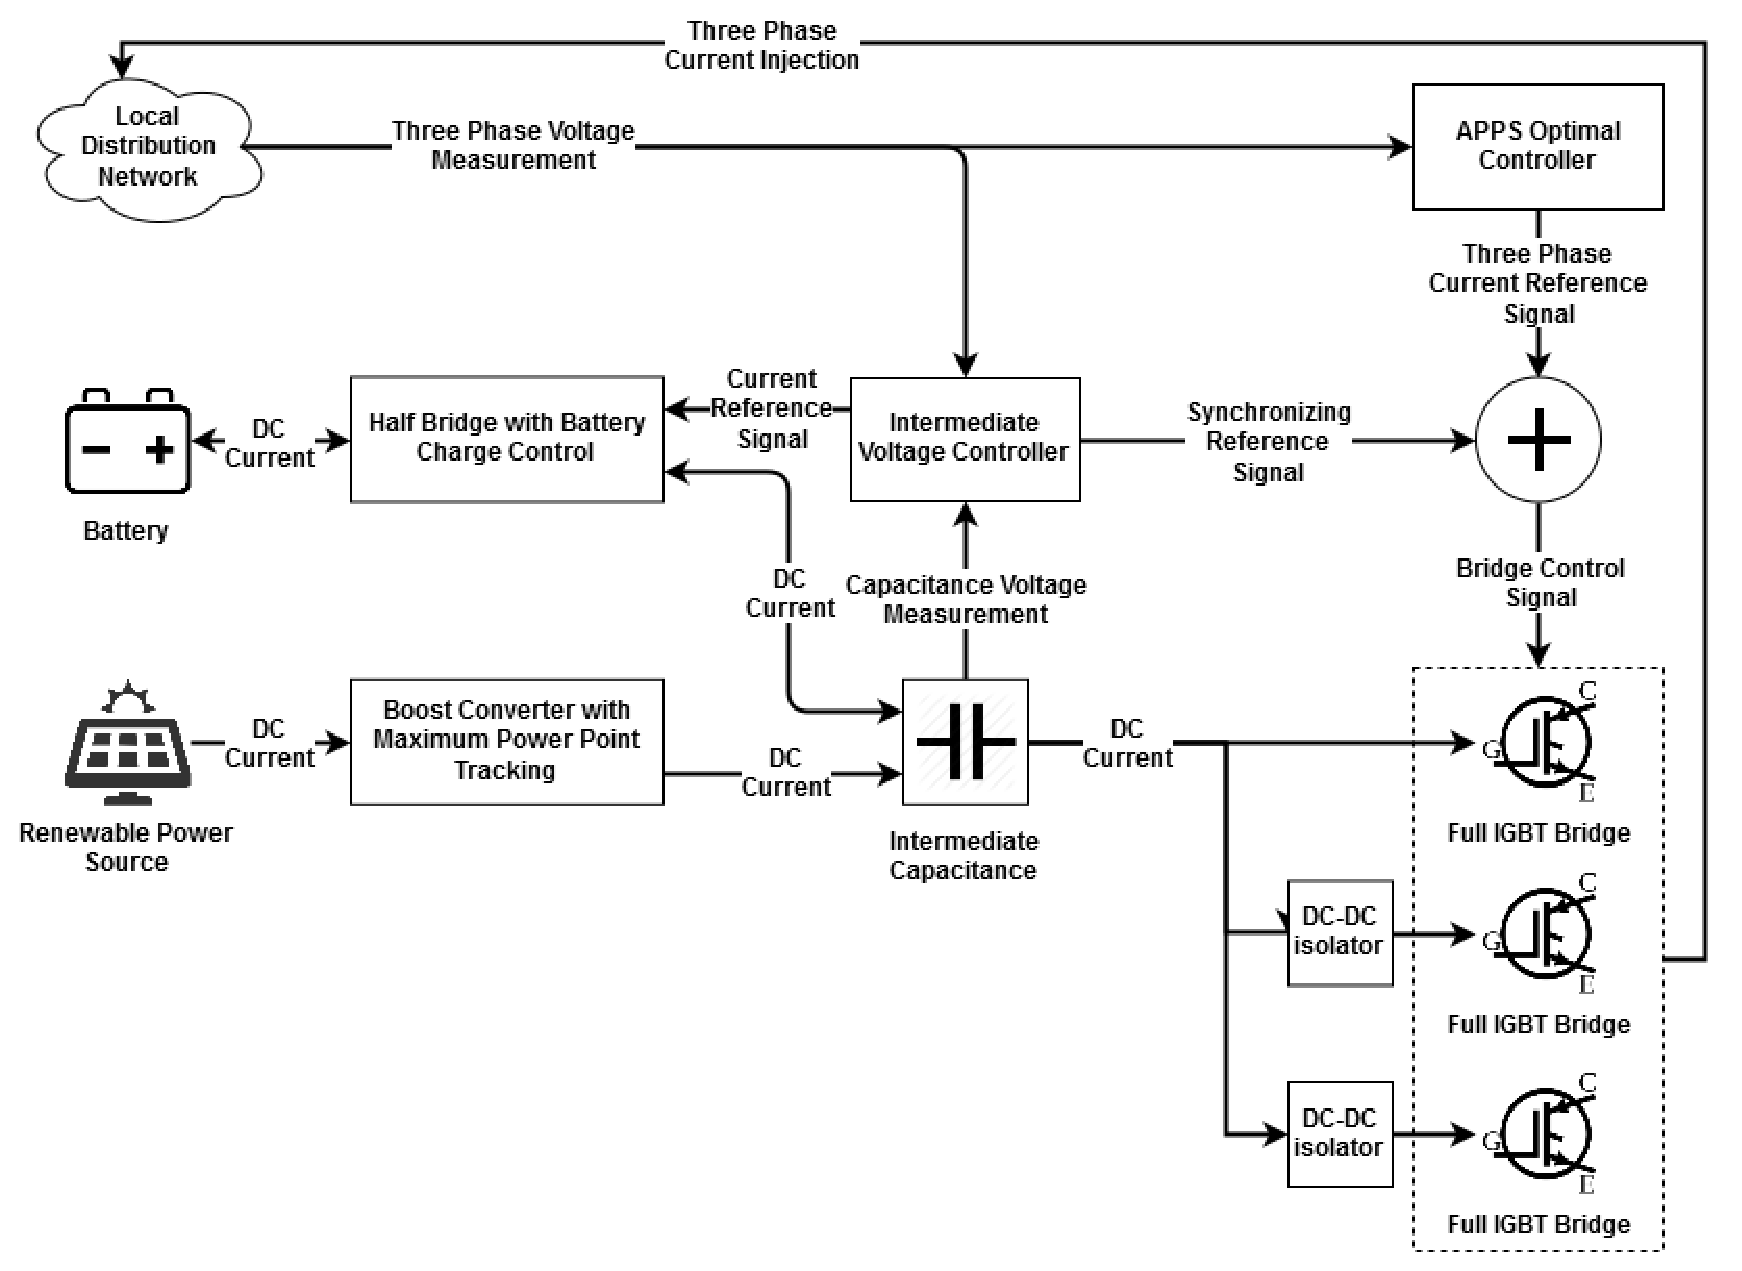
\includegraphics[width=0.95\textwidth]{Unblance_EPS_Pics/inverter.eps}
%        \caption{\textcolor{blue}{The asymmetrical inverter design, which applies three single phase full bridge IGBT current injector to create the injected asymmetrical current shapes for voltage unbalance compensation. }}
%        \label{fig:inv}
%        \end{figure*}
%
%    \textcolor{blue}{
%        Of course there is a possibility that there is no renewable power available for a longer period of time and the battery completely looses its charge. In this case the system should work merely with the power of the connection point but with  zero energy balance. This states to operate two controller with semi-opposite control goals. The optimization based controller requires current injection while the intermediate voltage controller (Figure \ref{fig:inv}) keeps the inverters energy balance. Although for this operation some of the control's performance should be sacrificed, unbalance compensation could be achieved even without external renewable power, and energy storage at a minimum power requirement.}
%        %\subsubsection{The necessity of switching the control off}
%%
%%                \textcolor{blue}{Inverter lea\'all\'it\'as\'anak sz\"uks\'egess\'ege.}
%
%%
%        The renewable energy injection is realized increasingly directly to the three phase low voltage grid in domestic size photovoltaic power plants too. This can reduce the voltage and current unbalance caused by the stochastic power production wind and solar sources. More and more manufacturers produce three phase grid synchronized inverters from 5\,kW size. These equipments implement symmetrical power feed with a standard three phase full bridge structure consists of six Isolated Gate Bipolar Transistors (IGBT). This is a cost effective standard structure suitable for symmetric harmonic current injection, but Kirchhoff's current law permits only constant zero-sum current time functions injected with this structure. The proposed control aim assumes the ability of injecting non constant zero-sum currents. As a further generalization step, the injection of no harmonic current shapes will be necessary in order to decrease the extant Total Harmonic Distortion (THD) of the network. These expectations yield an inverter with new structure suitable for arbitrary current injections without limitations. The design lends similar elements like in \cite{gorbe2012reduction} by means of battery charge, renewable power point tracking, intermediate voltage, and IGBT bridge control, but in this case the problem requires a three phase solution for the voltage unbalance reduction. The applied structure based on a full bridge IGBT structure used in single phase current injection. Three different IGBT full bridge were connected at the output point, thus our structure has three phase and neutral connection too, to carry out any current form. The disadvantage of this structure is that it needs 12 IGBTs in the output stage as opposed to the 6 IGBTs needed for a classical full bridge structure and needs three galvanically isolated direct current (DC) voltage source for feeding. \\
%        The other standard elements, that the inverter design consists:
%        \begin{itemize}
%            \item Standard maximum power point tracking (MPPT) input stage, to inject the maximum available power from the renewable source to the intermediate voltage capacitor with a simple controlled boost converter
%            \item A half bridge current controller to charge or deploy the battery pack connected to the complex energetic system for energy storage and energy unbalance compensation
%            \item Intermediate voltage controller
%            \item Universal three phase output stage with 3 single phase full bridge IGBT current injector and 2 high current DC-DC converter
%        \end{itemize}
%        This is suitable to inject any necessary current shape to the low voltage three phase grid connection even DC currents too. Later a power loss and production cost analysis will be necessary if the built structure will be suitable for asymmetric compensation of low voltage transformer area.
%
%        %\begin{figure*}[ht]
%%        \centering
%%        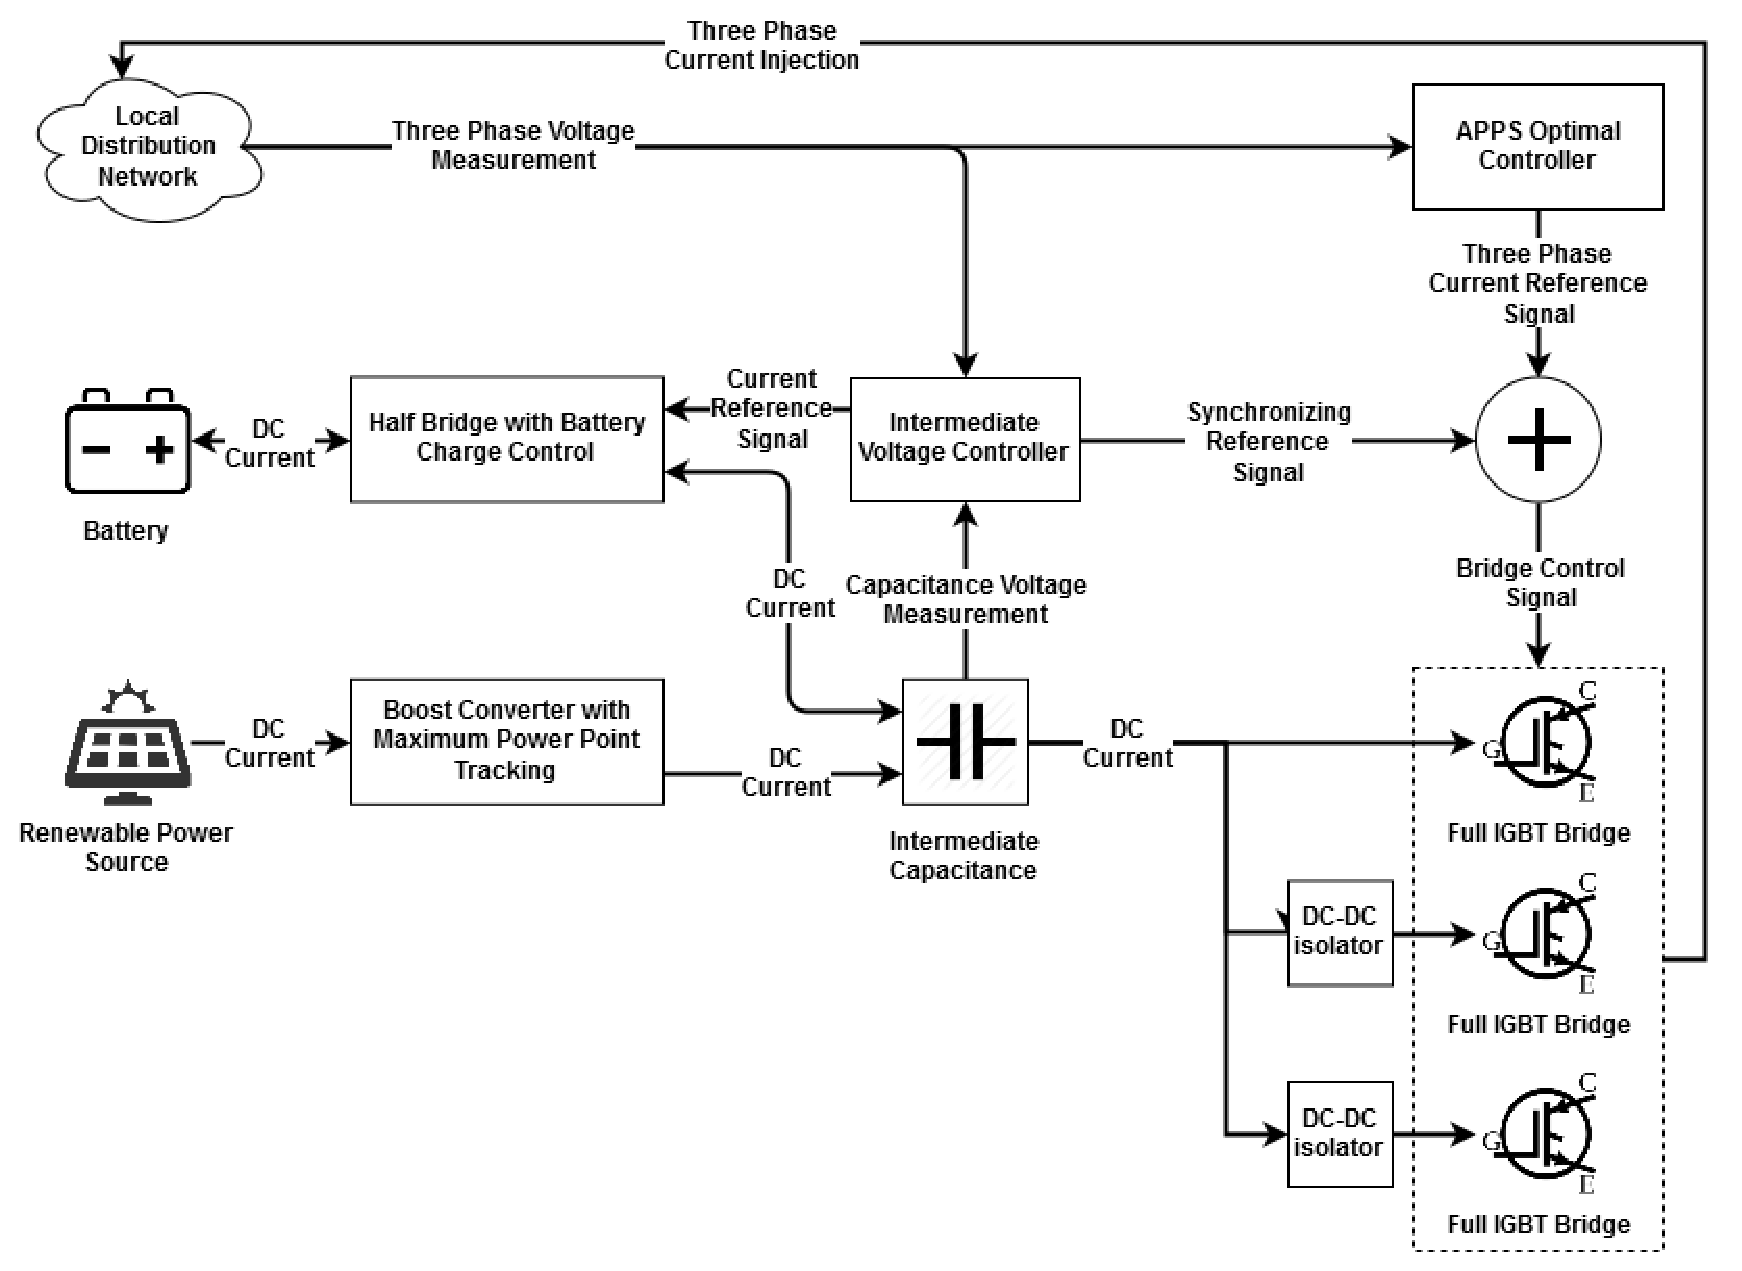
\includegraphics[width=0.95\textwidth]{Unblance_EPS_Pics/inverter.eps}
%%        \caption{The asymmetrical inverter design, which implies 3 single phase full bridge IGBT current injector to form the injected asymmetrical current shapes for voltage unbalance compensation. }
%%        \label{fig:inv}
%%        \end{figure*}
%%
%        Of course there is a possibility that there is no renewable power available for a longer period of time and the battery completely looses its charge. In this case the system should work merely with the power of the connection point but with  zero energy balance. This states to operate two controller with semi-opposite control goals. The optimization based controller requires current injection while the intermediate voltage controller (Figure \ref{fig:inv}) keeps the inverters energy balance. Although for this operation some of the control's performance should be sacrificed, unbalance compensation could be achieved even without external renewable power, and energy storage at a minimum power requirement.
%        %\subsubsection{The necessity of switching the control off}
%%
%%                \textcolor{blue}{Inverter lea\'all\'it\'as\'anak sz\"uks\'egess\'ege.}
%
%        \subsubsection{Measurements from a real unbalanced network}
%
%            The measurements took place at the Faculty's building, where a common 400\,V connection point was investigated as the behaviour of the network. The three phase 230\,V line-to-ground voltages has been transformed to 6\,V to be effectively measurable time domain with high performance NI-USB DAQ on 10\,ksample/s. Because of the limited computational capacity only a 10 second measurement was made in every hour.  The measurements then has been merged and smoothed to eliminate the inter-measurement transients.\\
%            Afterwards, the measurement data has been used as the output of a micro-grid segment of the Matlab/Simulink model, to test the controller and inverters structure's performance in quasi-realistic circumstances. The controllers performance on the simulated microgrid's network loss reduction can be observed on (Figure \ref{fig:compare_power}). The measurement output is connected to a modeled three phase load and network system, consisting of symmetrical loads and network segments between them. Further artificial load unbalance is not necessary since the network's unbalance is already present. This structure enables to show that any point the inverter is connected could serve as quality restoration such unbalance compensation at this case. Our future plan is to set up multiple devices on different connection points.
%
%
%
%    \subsection{Optimization based control algorithm}
%
%        \begin{figure*}[ht]
%        \centering
%        \includegraphics[width=0.95\textwidth]{Unblance_EPS_Pics/APPS_grey.eps}
%        \caption{\textcolor{blue}{The optimization algorithm implemented for current control. A one dimensional linear optimization step is being solved in each dimension of the six dimensional parameter space, iteratively.}}
%        \label{fig:APPS}
%        \end{figure*}
%
%        The problem is that, the exact mathematical relation is nonlinear because the nonlinear, and highly time variant loads of the network, we should use a control strategy to cope this nonlinear and time variant energy system. For this purpose we chose an asynchronous parallel pattern search method (APPS) which could be able to control our scenario.  We applied a variant of the gradient method that is a first-order optimization (minimization) algorithm for a multivariate function $f(x)$. The point $x(k)$ corresponding to the local minimum can be calculated from the negative gradient $\delta f(x)$, that gives the value and direction of the corresponding step in the parameter space. The next step is made in the direction of gradient with the proper sign. This sequence of steps, ideally, converges to local multivariate extreme value $x(k)$ of the function (\ref{eqn:contstruct1}).
%
%        \begin{equation}
%        \begin{array}{rcl}
%        \label{eqn:contstruct1}
%         x^{(k)}&=&x^{(k-1)}-t_k \nabla f(x^{(k-1)})\\
%         k&\in&\mathbb{N}\\
%         \end{array}
%        \end{equation}
%
%        The controlled electrical system is described by multivariate non-linear differential equations, the optimization of which is infeasible to derive using the differentiation of an error function. Therefore, the optimization methods based on direct differentiation are not applicable. In such cases, when high computational power is needed for performing long time-consuming simulations, the APPS method can utilized. The search pattern $p$ is based on the sampling of the error function (selected norm) on a "grid", and it corresponds to variables or subsets of variables in each point in the independent variable or parameter space easily. At the same time, the norm values at these points can be calculated independently if $\Delta k>0$, using (\ref{eqn:contstruct2}).
%        \begin{equation}
%        \label{eqn:contstruct2}
%        \begin{array}{rcl}
%         x^{(k+1)}&=&x^{(k)}+\Delta _kd_i \\
%         \mathrm{if}&&f(x^{(k)}+\Delta _kd_i) \leq f(x^{(k)})\\
%         k&\in&\mathbb{N}\\
%         \end{array}
%        \end{equation}
%
%        The parameter is  $x(k)\in R_n$, and the search pattern $p\in D={d_1,...d_n}$ is taken from a predefined finite set. In this case, the error function values should be calculated for each pattern $p$ in the set $D$. If the error function is not decreasing in any of the directions, then the step size should be reduced (e.g. by half). As the competing directions are different, if there is not enough computing power available for direction vector $p$, synchronization should not be maintained. In this case we are talking about the asynchronous case . In the case of our controller, an individual $p$ vector is defined for each output variable, and the optimization was performed in each direction asynchronously and shifted in time. Most likely, the error function has a single local minimum as a symmetric amplitude and phase values. Approaching the minimal value of norm, the controller uses adaptive increments that are proportional to the norm itself. Because of the complex interactions between the components of the controller, only one parameter is changed at a time, even if the values of the amplitude and phase components in specific time slot changes. The algorithm moves along the six axes of six separate time slots close to the local minimum of the error function.\\
%        Unlike other similar approaches, e.g. \cite{segui2007approach}, the explained optimal controller does not rely on a measured current signal but rather measuring and analysing the voltage unbalance via the proposed indicator and optimizes the voltage shape, the latter of which depends on the nonlinear distortion of the whole low-voltage transformer area and determines additional power losses. The controller's performance was compared to a non compensated network, and a network consisting synchronised symmetric power intake from a regular inverter.\\
%        In each iteration only one physical value is changing on the six dimensional parameter field, which consists of the three amplitude and three phase values. If the change effects with cost function reduction (the reference norm's normalised value), the controller holds the new value of amplitude or phase for the controlled current sources. The advantage of this controller structure that is not necessary to know the controlled value's behaviour well, like we could not determine the number and type of the other loads on the network \cite{Neukirchner2015}. There are however two disadvantages. First is the low speed of control, due to the several necessary iterations (depending on the circumstances) to find the optimal directions in the parameter space, and the serial nature of interventions and norm calculations. The second comes from the method itself since the controller may stuck in local minima.
%
%    %\subsubsection{Higher level control structure}
%%
%%            \begin{itemize}
%%            \item \textcolor{blue}{Norm\'al \'es z\'er\'o energimam\'erleg \"uzemm\'odok.}
%%            \item \textcolor{blue}{\"Uzemm\'od v\'altasok.}
%%            \end{itemize}
%
%\subsection{Discussion}
%    \subsubsection{Dynamical simulation based experiments}
%    In order to be able to investigate the proposed optimization based unbalance reduction control structure with the three phase inverter on a low voltage local grid, all the elements of this complex electrical system (including the photovoltaic source, the inverter, the battery and the nonlinear local grid with different types of loads) has been modeled in Matlab/Simulink environment. The primary aim of the simulation based experiments were to serve as a proof of concept for the proposed complex control structure.
%    \subsubsection{Performance analysis}
%    The aim of performance analysis is twofold. First of all, the proposed voltage unbalance indicator has to be investigated in the control structure as the cost function of the optimization based controller, and on the other hand, the control structure itself has to be exposed against engineering expectations.
%
%%     The first experiment is depicted in Figure \ref{fig:compare_asym_VEC}, where the vectorial based voltage unbalance indicator was used as the cost function of the optimization algorithm. The results are far not promising since the value of norm $N$ of the network starts to oscillate when the unbalance reduction controller is active. The cause of this behaviour is \textcolor{red}{WHAT?}
%%
%%             % V ==========================
%%            \begin{figure*}[h]
%%             \centering
%%                  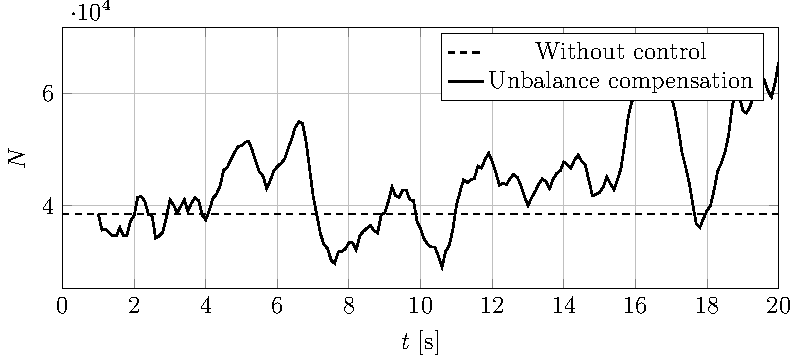
\includegraphics{UnbalRedComp_JCP-figure2.pdf}
%% %                 \pgfplotsset{every tick label/.append style={font=\normalsize}}
%% %                 \begin{tikzpicture}
%% %                 \begin{axis}[
%% %                     width=\textwidth,
%% %                     height=6cm,
%% %                     xlabel = {$t$~[s]},
%% %                     ylabel = {$N$},
%% %                     grid=major,
%% %                     xmin=0,
%% %                     xmax=20,
%% %                     %ymax=8000,
%% %                     %ymin=200,
%% %                     ]
%% %                     \addplot [dashed, thick] coordinates {(0,38520) (20,38520)};
%% %                     \addplot[thick] table {VEC_Measurements/VEC_orig.dat};
%% %                     \legend{Without control, Unbalance compensation}
%% %                     \end{axis}
%% %                  \end{tikzpicture}
%%                  \caption{Compensation control's voltage unbalance reduction, where $N$ indicates the calculation with the vectorial indicator value. The controller starts at $t=0.1s$ and starts oscillating towards unbalance.}
%%                  \label{fig:compare_asym_VEC}
%%                 \end{figure*}
%
%                The results of the first experiment can be seen in Figure \ref{fig:compare_asym_PV} where the geometrical norm \ref{equ:geom} has been used as the voltage unbalance indicator and the cost function for the optimizer.  The dashed line represents the examined low voltage local network's unbalance norm ($G$) without the proposed controller implemented in the inverter unit of the domestic powerplant while the solid line represents the compensated network'snorm value. The performance of the controller with this norm is apparent, it was able to decrease the network voltage unbalance by approximately 85 \%. In this experimental setup the controller has enough input energy due to the batteries and the available solar power.
%
%            % G ========================== +PV
%            \begin{figure*}[ht]
%            \centering
%            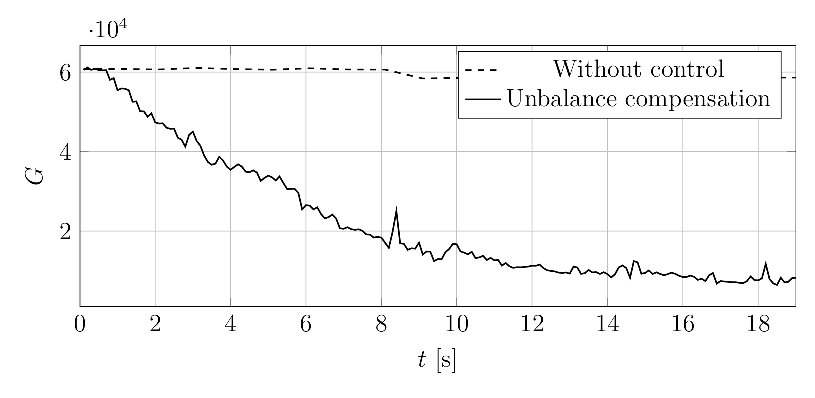
\includegraphics[width=0.95\textwidth]{Unblance_EPS_Pics/UnbalRedComp_JCP-figure3.eps}
%%                 %\pgfplotsset{every tick label/.append style={font=\tiny},legend style={at={(1,1)},anchor=north east}}
%%                 \pgfplotsset{every tick label/.append style={font=\normalsize}}
%%                 \begin{tikzpicture}
%%                 \begin{axis}[
%%                     width=\textwidth,
%%                     height=6cm,
%%                     xlabel = {$t$~[s]},
%%                     ylabel = {$G$},
%%                     grid=major,
%%                     xmin=0,
%%                     xmax=19,
%%                     %ymax=900,
%%                     %ymin=200,
%%                     ]
%%                     \addplot[dashed,thick] table {withPV/GEO_nocont_orig.dat};
%%                     \addplot[thick] table {withPV/GEO_orig.dat};
%%                     \legend{Without control, Unbalance compensation}
%%                     \end{axis}
%%                  \end{tikzpicture}
%                 \caption{Unbalance reduction control system performance with half charged battery and photovoltaic power source available. The underlying unbalance norm is the geometrical one ($G$) in this experiment. After starting the controller at $t=0.1s$ the unbalance measure $G$ of the network significantly decrease.}
%                 \label{fig:compare_asym_PV}
%                \end{figure*}
%
%                % G ========================== -PV
%            \begin{figure*}[ht]
%            \centering
%            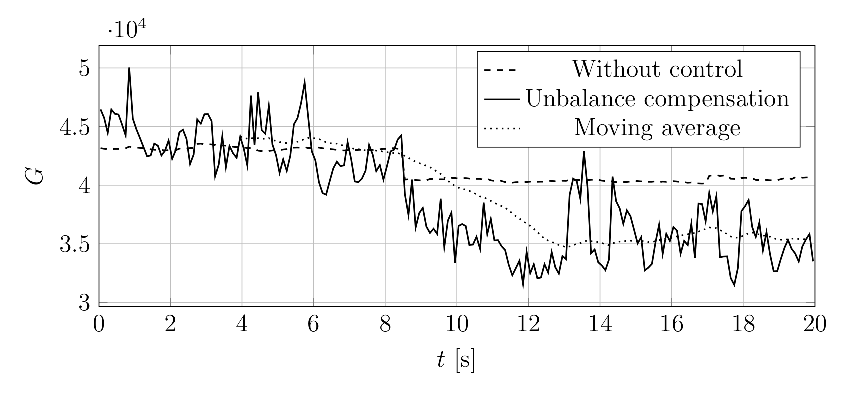
\includegraphics[width=0.95\textwidth]{Unblance_EPS_Pics/UnbalRedComp_JCP-figure4.eps}
%%                  %\pgfplotsset{every tick label/.append style={font=\tiny},legend style={at={(1,1)},anchor=north east}}
%%                 \pgfplotsset{every tick label/.append style={font=\normalsize}}
%%                 \begin{tikzpicture}
%%                 \begin{axis}[
%%                     width=\textwidth,
%%                     height=6cm,
%%                     xlabel = {$t$~[s]},
%%                     ylabel = {$G$},
%%                     grid=major,
%%                     xmin=0,
%%                     xmax=20,
%%                     %ymax=600,
%%                     %ymin=200,
%%                     ]
%%                     \addplot[dashed,thick] table {netw_plot_nocont/GEO_nocont_orig.dat};
%%                     \addplot[thick] table {netw_plot/GEO_orig.dat};
%%                     \addplot[dotted,thick] table {netw_plot/GEO_orig_mean.dat};
%%                     \legend{Without control, Unbalance compensation, Moving average}
%%                     \end{axis}
%%                  \end{tikzpicture}
%                 \caption{Unbalance reduction control system performance without battery and renewable source (zero energy balance operation). The performance reduction is clearly observable compared to the case when external power source is available (Figure \ref{fig:compare_asym_PV}), but as result the voltage unbalance indicator $G$ reduced by the average value of 14.78\%.}
%                 \label{fig:compare_asym}
%                \end{figure*}
%
%            A slightly more challangeing situation is investigated in Figure \ref{fig:compare_asym} where the controller had had to operate without photovoltaic source and batteries. This is called zero balance operation mode when the energy obtained from the network is reinjected in such a way that the unbalance indicators decrease. It can be seen that the performance of the controller is modest than that of Figure \ref{fig:compare_asym_PV}, but it is still acceptable.
%
%      \paragraph{Robustness analysis}
%
%            %\textcolor{magenta}{MACI}\\
%            %\textcolor{blue}{Robosztuss\'agi vizsg\'alat mind norm\'al mind zero balance esetre.}
%            The robustness of the proposed control structure is an important qualitative property with respect to the time dependent loads present on the network. The robustness of the proposed controller had to be tested via simulation when different types of loads (inductive, capacitive, resistive) had been varied in step changes representing represnting the on/off switching the different types of household appliances (motors, switching mode power supplies, electric heaters, stc.). In the experiment depicted in Figure \ref{fig:robustness}, a load change has been introduced to the network in every 15 seconds causing the voltage unbalance to jump to a different value (measured in the geometrical norm (\ref{equ:geom})). As it can be seen in the figure the controller successfully compensates the unbalance after each transient.
%
%              \begin{figure*}[ht]
%            \centering
%            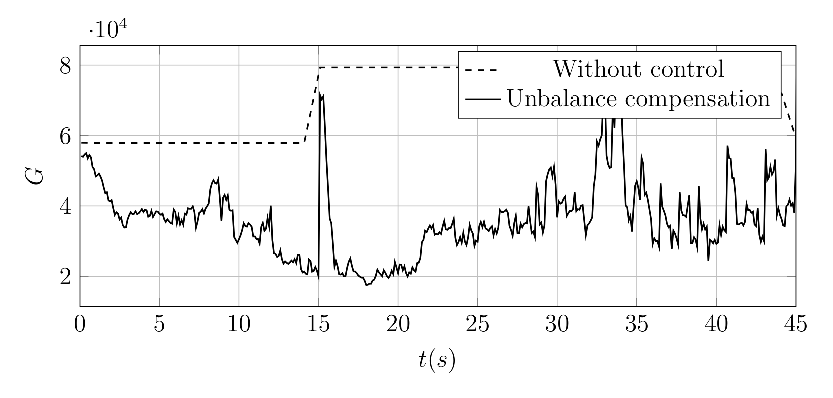
\includegraphics[width=0.95\textwidth]{Unblance_EPS_Pics/UnbalRedComp_JCP-figure5.eps}
%%             %\pgfplotsset{every tick label/.append style={font=\tiny},legend style={at={(1,1)},anchor=north east}}
%%             \pgfplotsset{every tick label/.append style={font=\normalsize}}
%%             \begin{tikzpicture}
%%             \begin{axis}[
%%             width=\textwidth,
%%             height=6cm,
%%             xlabel = {${t(s)}$},
%%             ylabel = {${G}$},
%%             grid=major,
%%             xmin=0,
%%             xmax=45,
%%             %ymax=140,
%%             ]
%%             \addplot[thick, dashed] table {robustness_nocont/GEO_nocont_orig.dat};
%%             \addplot[thick] table {robustness_regular/GEO_orig.dat};
%%             \legend{Without control, Unbalance compensation}
%%             \end{axis}
%%             \end{tikzpicture}
%            \caption{Robustness analysis with respect to step type changes in the network load (and voltage unbalance). The unbalance reduction controller successfully compensates the changes in the network voltage unbalance norm ($G$) value.}
%            \label{fig:robustness}
%            \end{figure*}
%
%
%
%    \subsubsection{Environmental effect}
%            favorable effects of the proposed unbalance reduction control algorithm , i.e. increase power quality not only at the connection point but in the whole low voltage transformer area, which causes a reduction of the effective power loss and the reduction in the CO${}_2$ emission.
%
%        \paragraph{Power loss reduction on the network}
%
%             Network loss reduction due to the unbalance reduction compensation control is investigated on Figure \ref{fig:compare_power} where the simulation experiment was carried out in the circumstance when the renewable source was not shut down (e.g. insufficient amount of sunlight) and additionally the battery was drained completely  \cite{Neukirchner2015}, \cite{neukirchner2015examination}.
%            \begin{figure*}[ht]
%            \centering
%            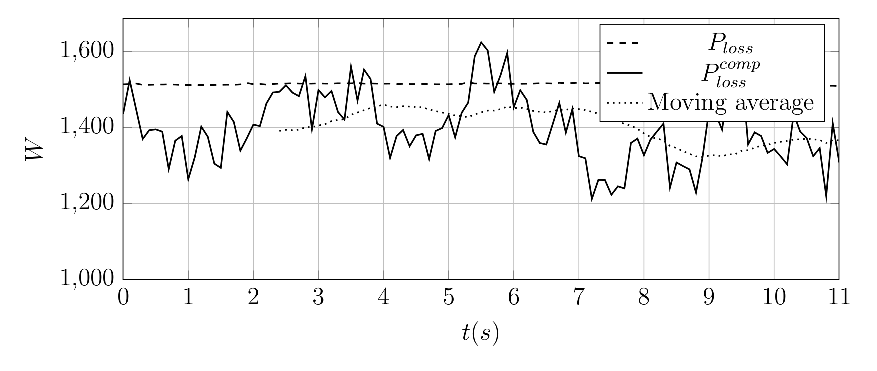
\includegraphics[width=0.95\textwidth]{Unblance_EPS_Pics/UnbalRedComp_JCP-figure6.eps}
%%             %\pgfplotsset{every tick label/.append style={font=\tiny},legend style={at={(1,1)},anchor=north east}}
%%             \pgfplotsset{every tick label/.append style={font=\normalsize}}
%%             \begin{tikzpicture}
%%             \begin{axis}[
%%             width=\textwidth,
%%             height=6cm,
%%             xlabel = {${t(s)}$},
%%             ylabel = {${W}$},
%%             grid=major,
%%             xmin=0,
%%             xmax=20,
%%             ymin=1000,
%%             ]
%%             \addplot[dashed,thick] table {netw_plot_nocont/P_loss.dat};
%%             \addplot[thick] table {netw_plot/P_loss.dat};
%%             \addplot[dotted,thick] table {netw_plot/P_loss_mean.dat};
%%             \legend{$P_{loss}$,$P^{comp}_{loss}$,Moving average}
%%             \end{axis}
%%             \end{tikzpicture}
%            \caption{Compensation control's loss reduction during zero energy balance operation on the modeled network, where $P_{loss}$ indicates the effective power losses and $P^{comp}_{loss}$ effective power losses during control of the network. As result the network losses reduced by mean $6.5\%$.}
%            \label{fig:compare_power}
%            \end{figure*}
%            The results show that despite of the negative cross effects of the intermediate voltage controller and the unbalance reduction controller it was possible to find the trade-off between the control goals of the different controllers (maintain zero energy balance for the inverter and decrease the unbalance on the network). The estimated loss reduction in the experimental setup is 6.5\%.
%            \begin{figure*}[ht]
%            \centering
%            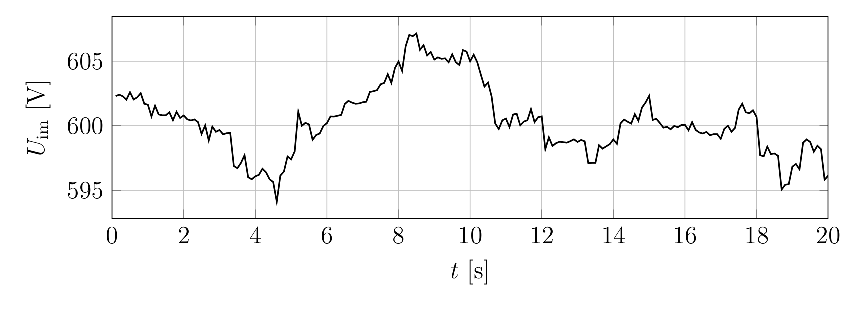
\includegraphics[width=0.95\textwidth]{Unblance_EPS_Pics/UnbalRedComp_JCP-figure7.eps}
%%                  %\pgfplotsset{every tick label/.append style={font=\tiny},legend style={at={(1,1)},anchor=north east}}
%%                 \pgfplotsset{every tick label/.append style={font=\normalsize}}
%%                 \begin{tikzpicture}
%%                 \begin{axis}[
%%                     width=\textwidth,
%%                     height=5cm,
%%                     xlabel = {$t$~[s]},
%%                     ylabel = {$U_{\textnormal{im}}$~[V]},
%%                     grid=major,
%%                     xmin=0,
%%                     xmax=20,
%%                     %ymin=0,
%%                     ]
%%                     \addplot[thick] table {netw_plot/U_inter.dat};
%%                     %\legend{\scriptsize$U_{intermediate}$}
%%                     \end{axis}
%%                  \end{tikzpicture}
%                 \caption{Intermediate puffer capacitance's voltage within boundaries ($600\pm10$\,V), during zero energy balance operation mode of the voltage unbalance compensation controller. $U_{\textnormal{im}}$ indicates intermediate the capacitance's voltage.}
%                 \label{fig:u_inter}
%                \end{figure*}
%
%        \paragraph[CO2 footprint]{CO$_2$ footprint}
%
%            The fact that this controller enables the reactive power reduction has a favourable consequence, i.e. the power loss or equivalently CO$_2$ emission and the carbon footprint can also be decreased. The estimated environmental effects of voltage asymmetry compensation can be calculated. Let us assume 3000\,kWh for the yearly electric energy consumption an average household and $9.173\%$ for the loss of the distribution network \cite{MVM2013}. With the controller the losses on the simulated network are reduced by 6.5\%. The calculation follows (\ref{eqn:co_emission})
%
%            \begin{equation}
%                \label{eqn:co_emission}
%                \begin{array}{rcl}
%                 P_{loss}&=&3000\,\textnormal{kWh}\cdot9.173\%\\
%                P^{comp}_{loss}&=&3000\,\textnormal{kWh}\cdot(9.173\cdot0.93)\%\\
%                 \Delta P_{loss}&=&P_{loss}-P^{comp}_{loss}\\
%                 \end{array}
%                \end{equation}
%
%            where $P_{loss}$ is the assumed network loss per household and $P^{comp}_{loss}$ is s the assumed network loss with unbalance compensation control and $\Delta P_{loss}$ is the saved energy. According to (\ref{eqn:co_emission}), unbalance compensation results in an energy savings of 19.26 kWh. Taking into account the proportion of power currently generated by fossil fuels (coal 17.3\,\%, gas 38.3\% \cite{MVM2013}, \cite{gorbe2012reduction}) and the rate of $\textnormal{CO}_2$ emission during electric energy production (1,000\,g/kWh from coal and 430\,g/kWh from gas), it can be concluded that voltage unbalance compensation could reduce $\textnormal{CO}_2$ emissions by 6504.9\,g a year, in an average household. %Note that this result reflect only the proof of concept, due the neglected power losses of the inverter and the artificial load of the network.
%
%
%\subsection{Conclusion}
%
%    The currently used measures of voltage unbalance has been extended in this work with a norm candidate. It is more demanding from the computational point of view but has an interesting feature namely it checks electrical asymmetry, i.e. the norm of a $\pm120$ degree  rotated version of the ideal three-phase phasor is zero in the geometrical sense.\\
%    The defined norm is applied as a cost function in the asymmetry reducing controller structure also presented in the paper. Simulations show that the geometrical based unbalance indicator can serve as a basis of further research. The suggested controller structure enables the residential users owning a grid synchronized domestic power plant to reduce voltage unbalance measurable at the connection point. The fundamental element of the system is a modified three phase inverter that is capable of the asymmetric injection of any current waveforms to the network. The optimization based control algorithm injects the available energy (as current waveform) in such a way, that the voltage unbalance decreases. This optimization problem is usually constrained by the available renewable energy supplied by the power plant.\\
%    The control structure has been tested on a low voltage network model in a dynamical simulation environment consisting of the models of the electrical grid, a domestic power plant,  asymmetrical inverter circuit, and different types of loads. Different simulation experiments has been run for each norm and for both the power constrained and unconstrained case. The preliminary results show that this structure can serve as a residential level voltage quality improvement method for the three phase low voltage network.

